%----------------------------------------------------------------------------------------
%	PACKAGES AND OTHER DOCUMENT CONFIGURATIONS
%------------------------------------------------------------------------
\documentclass[11pt]{article}
\usepackage[utf8]{inputenc} % Required for inputting international characters
\usepackage[T1]{fontenc} % Output font encoding for international characters
\usepackage{mathpazo} % Palatino font
\usepackage[czech]{babel} % Czech
\usepackage{graphicx}  % Graphics
\usepackage{caption}  % Caption
%\usepackage[amsmath]
\usepackage{placeins}

\begin{document}

%----------------------------------------------------------------------------------------
%	TITLE PAGE
%----------------------------------------------------------------------------------------

\begin{titlepage} % Suppresses displaying the page number on the title page and the subsequent page counts as page 1
	\newcommand{\HRule}{\rule{\linewidth}{0.5mm}} % Defines a new command for horizontal lines, change thickness here
	
	\center % Centre everything on the page
	
	%------------------------------------------------
	%	Headings
	%------------------------------------------------
	
	\textsc{\LARGE České vysoké učení technické v Praze}\\[1.5cm] % Main heading such as the name of your university/college
	
	\textsc{\Large Algoritmy digitální kartografie a GIS}\\[0.5cm] % Major heading such as course name
	
	\textsc{\large Katedra geomatiky}\\[0.5cm] % Minor heading such as course title
	
	%------------------------------------------------
	%	Title
	%------------------------------------------------
	
	\HRule\\[0.4cm]
	
	{\huge\bfseries Úloha č. 3: Digitální model terénu}\\[0.4cm] % Title of your document
	
	\HRule\\[1.5cm]
	
	%------------------------------------------------
	%	Author(s)
	%------------------------------------------------
	
	

	
	% If you don't want a supervisor, uncomment the two lines below and comment the code above
	Monika \textsc{Křížová} % Your name
	
	Marek \textsc{Hoffmann}
	
	%------------------------------------------------
	%	Date
	%------------------------------------------------
	
	\vfill\vfill\vfill % Position the date 3/4 down the remaining page
	
	{\large 4.12.2021} % Date, change the \today to a set date if you want to be precise
	
	%------------------------------------------------
	%	Logo
	%------------------------------------------------
	
	%\vfill\vfill
	%\includegraphics[width=0.2\textwidth]{placeholder.jpg}\\[1cm] % Include a department/university logo - this will require the graphicx package
	 
	%----------------------------------------------------------------------------------------
	
	\vfill % Push the date up 1/4 of the remaining page
	
\end{titlepage}

%----------------------------------------------------------------------------------------


%----------------------------------------------------------------------------------------
%	TABLE OF CONTENT
%----------------------------------------------------------------------------------------

\tableofcontents
%\thispagestyle{empty}

\clearpage

%----------------------------------------------------------------------------------------
%	ZADÁNÍ
%----------------------------------------------------------------------------------------

\section{Zadání}
Navrhněte aplikaci s grafickým rozhraním, která nad množinou bodů vytvoří polyedrický digitální model terénu.

Jako vstupní data využijte existující data o alespoň 300 bodech. Nad nimi vytvořte Delaunayovu triangulaci metodou inkrementální konstrukce. Triangulaci využijte pro výpočet a vykreslení vrstevnic. Výslednou triangulaci doplňte o vhodnou vizualizaci sklonu jednotlivých trojúhelníků a jejich expozici. 

%----------------------------------------------------------------------------------------
%	BONUSOVÉ ÚLOHY
%----------------------------------------------------------------------------------------

\section{Údaje o bonusových úlohách}
Zpracovány byly celkem 3 bonusové úlohy ze 7 zadaných.

\begin{itemize}
	\item Triangulace nekonvexní oblasti zadané polygonem +5b
	\item Výběr barevných stupnic při vizualizaci sklonu a expozice. +3b
	\item Automatický popis vrstevnic respektující kartografické zásady +10b - z části
	
\end{itemize}

%----------------------------------------------------------------------------------------
%	POPIS PROBLÉMU
%----------------------------------------------------------------------------------------

\section{Popis problému}
Triangulace je jednou ze základních výpočetních úloh nejen v oblasti digitální kartografie. Kromě tvorby DMT své uplatnění najde i při tvorbě jakékoliv vizualizace prostorových dat ve formě 3D modelů. Dále lze triangulaci využít při detekci otisku prstů či např. modelování přírodních jevů.
 
\subsection{Formulace problému}

Mějme množinu bodů $P$. Triangulací se rozumí převod množiny bodů na trojúhelníkovou síť $m$ trojúhelníků $t$ tak, aby platilo:

\begin{itemize}
	\item Libovolné 2 trojúhelníky mají společnou nejvýše jednu hranu.
	\item Sjednocení trojúhelníků je souvislá množina.
	\item Uvnitř žádného trojúhelníku neleží žádný další bod z $P$.	
\end{itemize}

Triangulace by měla tvořit pravidelné trojúhelníky blížící se trojúhelníkům rovnostranným a všechny trojúhelníky by se v každém bodě měly co nejlépe přimykat terénu. 

%----------------------------------------------------------------------------------------
%	POPIS ALGORITMŮ
%----------------------------------------------------------------------------------------

\section{Popisy algoritmů}
\subsection{Delaunayova triangulace}

Existuje několik druhů triangulace. Nejpoužívanější je však Delaunayova triangulace, která svými kritérii zajišťuje jednoznačnost, spolehlivé výsledky a má optimální časovou složitost. Tyto požadavky jsou následující:

\begin{itemize}
\item Uvnitř kružnice $k$ opsanému libovolnému trojúhelníku $t_{j}$ neleží žádný jiný bod množiny $P$.
\item $DT$ maximalizuje minimální úhel v každém $t_{j}$, ale neminimalizuje maximální úhel v $t_{j}$. 
\item $DT$ je lokálně i globální optimální vůči kritériu minimálního úhlu.
\item $DT$ je jednoznačná, pokud žádné 4 body neleží na kružnici.

\end{itemize}

\subsubsection{Inkrementální konstrukce}
Existuje několik metod konstrukce Delaunayho triangulace. V této úloze však byla implementována metoda inkrementální konstrukce, která je založena na postupném přidávání bodů do již vytvořené triangulace.

Pro konstrukci je používána datová struktura AEL (Active Edge List), která obsahuje hrany $e$, ke kterým hledáme Delaunayovský bod minimalizující poloměr kružnice mezi Delaunayovskou hranou a hledaným bodem. Delaunayovská hrana je orientovaná a bod hledáme pouze vlevo od ní.

 \paragraph{Popis Algoritmu}
 
 \begin{enumerate}
 \item Nalezení bodu $q$ s nejmenší x-ovou souřadnicí $$ q = min(x_i) $$ 
 \item Nalezení nejbližšího bodu k počátečnímu bodu $$ ||p_1 - q||_2 = min  $$
 \item Vytvoření první hrany $$ e = (q, p_1) $$
 \item Hledání Delaunayho bodu $$ \underline{p} = argmin_{\forall p_i \in \sigma_L (e)} r'(k_i); k_i = (a, b, p_i); e = (a, b)$$
 \item Při neexistenci Delaunayho bodu změna orientace hrany a opakování předchozího kroku $$ \not\exists \underline{p} : e \leftarrow (p_1, q);$$ 
 \item Vytvoření zbývajících hran trojúhelníka  $$ e_2 = (p_1,  \underline{p}); e_3 = ( \underline{p} , q) $$
 \item Přidání hran do AEL  $$ AEL \leftarrow e; AEL \leftarrow e_2; AEL \leftarrow e_3  $$  
 \item Přidání hran do DT   $$ DT \leftarrow e; DT \leftarrow e_2; DT \leftarrow e_3  $$
 \item Dokud není vektor AEL prázdný: 
 
		Změna orientace první hrany z AEL $$ e = (p_1, q) $$
		Hledání Delaunayho bodu k e  $$ \underline{p} = argmin_{\forall p_i \in \sigma_L (e)} r'(k_i); k_i = (a, b, p_i); e = (a, b)$$ 
		Pokud bod existuje $$ if \exists  \underline{p}$$
		Tvorba zbývajících hran trojúhelníku $$ e_2 = (p_2,  \underline{p}); e_3 = ( \underline{p} , q) $$
		Přidání hran do DT $$ DT \leftarrow e; DT \leftarrow e_2; DT \leftarrow e_3  $$
		Přidání hrany do AEL, pokud již neexistuje s opačnou orientací.$$AEL if \not\exists \leftarrow e_2; AEL \leftarrow e_3  $$ 
 \end{enumerate}

\subsection{Delaunayova triangulace nekonvexního polygonu}
Konstrukce Delaunayovy triangulace nekonvexního polygonu je téměř totožná s triangulací tachymetrie. Jedinou výjimkou je nutnost odebrání trojúhelníků s těžištěm ležícím mimo polygon. 

Těžiště trojúhelníku se vypočte jako průměr souřadnic vrcholů trojhúhelníku. Pro zjištění, zda leží bod (těžiště) uvnitř polygonu byla použita metoda Winding number algoritmu, jež byla konstruována v první úloze tohoto předmětu, v jejíž dokumentaci je algoritmus podrobně vysvětlen.

\subsection{Konstrukce vrstevnic lineární interpolací}
Vrstevnice je křivka, která spojuje body se stejnou nadmořskou výškou. Zpravidla bývají vrstevnice vykreslovány s pravidelným intervalem.

Vrstevnice dělíme na základní a hlavní. Základní vrstevnice tvořené s pravidelným základním intervalem bývají vyznačeny tenkou, nepřerušovanou linií a jsou uzavřené. Hlavní vrstevnice je každá pátá základní vrstevnice. V mapách bývá značena tlustou, nepřerušovanou, uzavřenou linií a bývají doplněny popisem.

Dále existují vrstevnice doplňkové, které doplňují základní vrstevnice v těch místech, kde dostatečně nevystihují zejména sklonitý terén, a vrstevnice pomocné, které se používají pro místa s nestálým reliéfem jako např. v oblastech povrchové těžby. Doplňkové ani pomocné vrstevnice nebyly v této aplikaci implementovány.

\subsubsection{Lineární interpolace}
Lineární interpolace předpokládá:
\begin{enumerate}
\item Spád terénu mezi dvěma body, mezi kterými provádíme interpolaci, je konstantní.
\item Rozestup vrstevnic mezi dvěma body je konstantní.
\end{enumerate}

Na vstupu máme trojúhelník $t$ a vodorovnou rovinu $\rho$ o výšce $h$. Lineární interpolace je založena na analytické geometrii. Hledáme tedy průsečnici roviny $T$ určené trojúhelníkem $t$ a vodorovnou rovinou. Tento výpočet provedeme nad každým trojúhelníkem $t$

\subsubsection{Algoritmus}

\begin{enumerate}
\item Nalezení průsečíků všech horizontálních rovin s jednotlivými hranami.

Varianty vzájemné polohy $\rho$ a $T$:
	\begin{enumerate}
		\item Nemají žádný společný bod - neřešíme.
		\item Průsečnice tvoří jeden bod - neřešíme.
		\item Průsečnice je úsečka:
		\begin{itemize}
		\item Hrana leží v rovině $\rho$ - vrstevnice je přímo v hraně.
		\item Průsečnice roviny s trojúhelníkem vytvářející nové průsečíky mezi vrcholy trojúhelníku - vrstevnice je vykreslena mezi body vypočtenými následujícími rovnicemi:
$$  x = \frac{(x_2 - x_1)}{(z_2 - z_1)} (z - z_1) + x_1 $$ 		
$$  y = \frac{(y_2 - y_1)}{(z_2 - z_1)} (z - z_1) + y_1 $$ 
		\end{itemize}
		\item Všechny hrany trojúhelníku leží v rovině $\rho$ - neřešíme.	
	\end{enumerate}

\end{enumerate}
 
\subsection{Algoritmus výpočtu sklonu trojúhelníku}
Sklon představuje jednu z analytických úloh realizovaných nad DMT. Určuje, zdali terén stoupá, klesá nebo je rovinný.

Sklon představuje úhel $ \varphi $ mezi svislicí a normálovým vektorem trojúhelníku. Vypočte se následujícím způsobem.

$$  u = (u_x, u_y, u_z)$$
$$  v = (v_x, v_y, v_z)$$
$$ n = \vec{u}\times \vec{v} = (n_x, n_y, n_z)$$
$$ \varphi = arccos \frac{n_z}{|n|} $$ 

Barevná vizualizace sklonu terénu je vytvořena pomocí interpolace jednotlivých složek barevného schématu RGB. Při tvorbě je vždy nejprve vypočten podíl sklonu trojúhelníku a sklonu maximálního. Tento podíl je následně násoben hodnotou 255 a poté je vždy buď uložen do složky barvy, nebo odečten od hodnoty 255, má-li klesat podíl této složky. 

Při volbě vizualizace sklonu (\textit{s}) v barvách mezi zelenou a červenou barvou je výpočet následující. Zelená barva má složky (0,255,0) a červená (255,0,255), proto je nutné, aby podíl zelené složky s rostoucím sklonem klesal a podíl červené složky naopak stoupal, podíl modré složky je vždy nulový. Výpočet tedy bude proveden následovně:

$$	x = \frac{s}{s_{max}} $$
$$	red = x*255 $$
$$	green = 255-x*255 $$
$$	blue = 0 $$

\subsection{Algoritmus výpočtu expozice trojúhelníku}
Expozice představuje orientaci terénu vzhledem ke Slunci.

Orientace v bodě je definován jako azimut průmětu normálového vektoru roviny trojúhelníku do roviny x,y.

$$  u = (u_x, u_y, u_z)$$
$$  v = (v_x, v_y, v_z)$$
$$ n_t = \vec{u}\times \vec{v} = (n_x, n_y, n_z)$$
$$ A =atan2( \frac{n_x}{n_y}) $$

Expozice je v případě barevného schématu zobrazována v následujícím barevném schématu.

\begin{figure}[htbh]
	\centering
	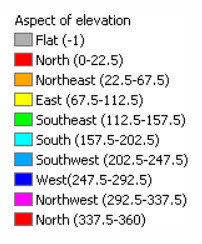
\includegraphics[scale=1]{images/expozice.jpg} 
	\caption{vizualizace expozice terénu}
	\label{fig:getExposition()}
\end{figure} 

\clearpage

%----------------------------------------------------------------------------------------
%	PROBLEMATICKÉ SITUACE
%----------------------------------------------------------------------------------------
\section{Problematické situace}
	
\subsection{Transformace souřadnic}
	Abychom mohli v oknu aplikace zobrazovat budovy, jejíž lomové body jsou určeny v souřadnicovém systému S-JTSK, bylo nutné souřadnic převést do souřadnicového systému widgetu. 
	
\subsubsection{Počátek}
	Pro určení souřadnic počátku bylo nejdříve nutno zjistit maximální hodnotu souřadnice Y a minimální hodnotu souřadnice X v souřadnicovém systému S-JTSK. 
	
\begin{figure}[htbh]
	\centering
	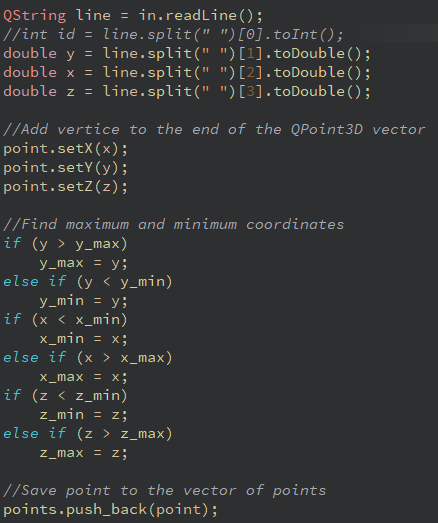
\includegraphics[scale=0.8]{images/U2_problem_pocatek.png} 
	\caption{Výpočet souřadnic počátku}
	\label{fig:problem_origin}
\end{figure} 
	
\subsubsection{Měřítko}
Abychom zobrazili pouze území, kde se polygony nachází, bylo nutné také zavést měřítko.
	
Měřítko jsme definovali jako podíl šířky/výšky widgetu ku rozdílu maximální a minimální souřadnici v dané ose. Bylo tedy nutné zjistit také minimální hodnotu souřadnice Y a maximální hodnotu souřadnice X.
	

Měřítko se následně vypočetlo v obou osách, a abychom zabránili tomu, že transformované souřadnice budou mít vyšší hodnotu, než je rozměr widgetu, použilo se měřítko s menším maximálním souřadnicovým rozdílem.
	
\begin{figure}[htbh]
	\centering
	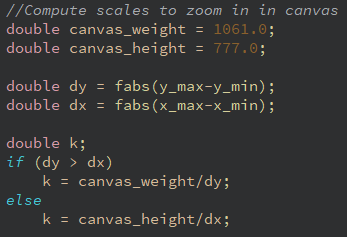
\includegraphics[scale=0.8]{images/U2_problem_meritko2.png} 
	\caption{Výpočet měřítka}
	\label{fig:problem_scale2}
\end{figure} 
	
\subsubsection{Transformace souřadnic}
Souřadnice v souřadnicovém systému widgetu byly definovány následujícími vzorci.	
	$$X_{W_{i}}=-k *\left(Y_{S-J T S K_{i}}-Y_{S-J T S K_{\max }}\right)$$	
	$$ Y_{W_{i}}=k *\left(X_{S-J T S K_{i}}-X_{S-J T S K_{\min }}\right)$$
	
\begin{figure}[htbh]
	\centering
	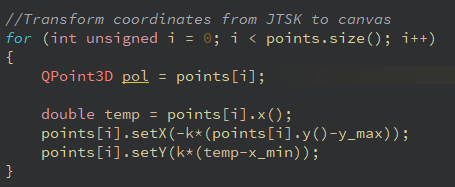
\includegraphics[scale=1]{images/U2_problem_transformace.png} 
	\caption{Transformace souřadnic}
	\label{fig:problem_transformation}
\end{figure} 

\clearpage

\subsection{Automatické určování maximální a minimální hodnoty z}
Aby nemusel uživatel ručně zadávat maximální a minimální hodnotu z, byla napsána funkce round2num(), která má na vstupu 3 parametry; zaokrouhlované číslo, násobek a směr.

Zaokrouhlované číslo představuje číslo, které chceme zaokrouhlit. Násobek je číslo, na jehož násobek chceme zaokrouhlované číslo zaokrouhlit. Směr je proměnná typu bool. Pokud je rovna true, zaokrouhlujeme nahoru, pokud je rovna false, zaokrouhlujeme dolů.

\begin{figure}[htbh]
	\centering
	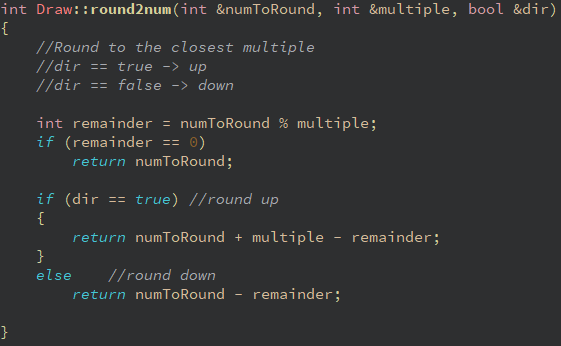
\includegraphics[scale=0.7]{images/round2num.png} 
	\caption{Funkce round2num()}
	\label{fig:round2num}
\end{figure} 

Ve funkci LoadData() tak nejdříve zjistíme extrémní hodnoty y, poté zaokrouhlíme na celá čísla a poté provedeme funkci round2num() jako zobrazuje následující obrázek.

\begin{figure}[htbh]
	\centering
	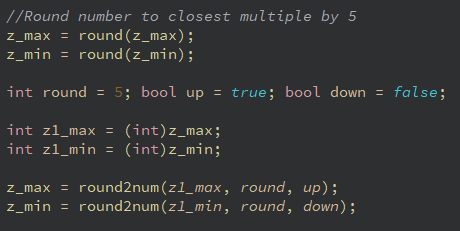
\includegraphics[scale=0.7]{images/round2num2.png} 
	\caption{Funkce aplikace round2num() v LoadData()}
	\label{fig:round2num2}
\end{figure} 

Jelikož chceme, aby se vrstevnice zobrazovaly ve výškách po pěti metrech, rovná se násobek pěti.

\subsection{Automatické generování popisu vrstevnic}
Výškovou kótou bývají popisovány hlavní vrstevnice. I popis by však měl dodržovat určité kartografické zásady.
\begin{itemize}
\item Kóty se umisťují tak, aby byly čitelné při pohledu ve směru stoupání.
\item Kóty se umisťují nepravidelně a rovnoměrně po celé ploše zobrazovaného území.
\end{itemize}

Nicméně, automatický popis vrstevnic respektující kartografické zásady byl v kódu implementován pouze z části. 

Ve třídě Algorithms se vytvořila funkce calculateLabelPoints(), která se volá po stisknutí tlačítka \textit{Create contours} se zaškrtnutým checkboxem \textit{Show contour labels}.

Na vstupu jsou vektor hran hlavních vrstevnic a množina bodů $P$. Výstupem funkce jsou vektor 3D bodů a vektor úhlů s datovým typem double. Funkce počítá souřadnice x a y bodu  uprostřed vrstevnice v každém patnáctém trojúhelníku, čímž je zajištěné nepravidelné a náhodné umístění výškových popisů. Z-ová souřadnice je převzána z počátečního bodu segmentu, neboť jejíž hodnota je pro celou vrstevnici konstantní. Ze souřadnicových rozdílů počátečního a koncového bodu každého segmentu vrstevnice je dále vypočtena směrnice přímky, podle které se následně budou orientovat popisy tak, aby byly rovnoběžné s vrstevnicemi.

$$ lp_x = ( \frac{s_x + e_x}{2});  lp_y = ( \frac{s_y + e_y}{2}) $$ 
$$ \epsilon = atan2( \frac{dy}{dx}) $$

\begin{figure}[htbh]
	\centering
	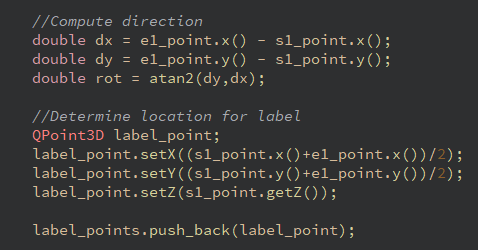
\includegraphics[scale=0.8]{images/getContourLabels.png} 
	\caption{výpočet souřadnic a směrnice bodu na popis průmky}
	\label{fig:getContourLines()}
\end{figure} 

Ve třídě Draw pak byly nejdříve vygenerovány obdélníky v barvě plátna, aby mohly být popisy umístěny přímo na vrstevnice a aby nebyly popisy vrstevnicemi rušeny. 

Abychom mohli vykreslit obdélníky ve směru vrstevnice, musíme nejdříve celý souřadnicový systém posunout do bodu vypočteného funkcí getContourLines() a pootočit o směrnici vypočtenou ze stejné funkce. V transformovaném souřadnicovém systému následně vykreslíme obdélník s vhodnými rozměry a souřadnicový systém transformujeme zpět do původního souřadnicového systému plátna.

\begin{figure}[htbh]
	\centering
	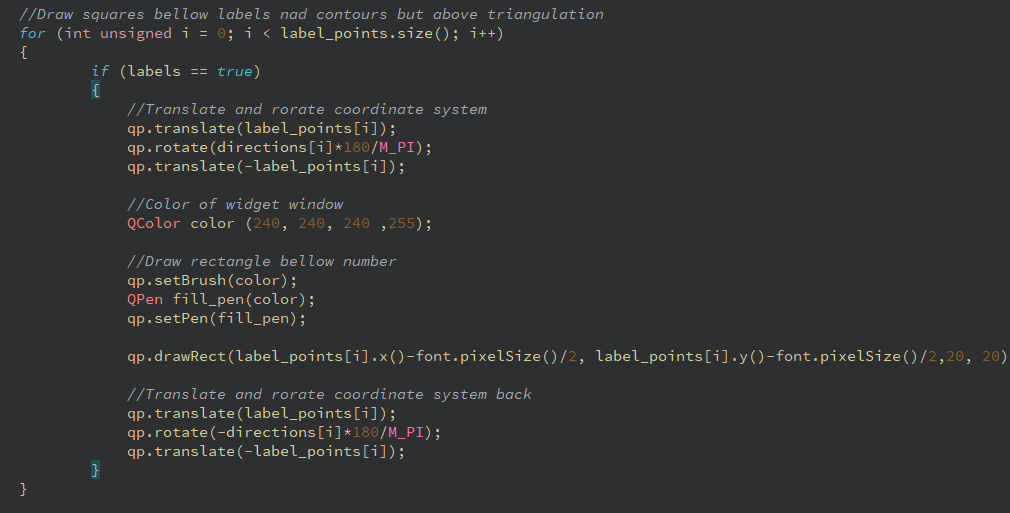
\includegraphics[scale=0.5]{images/DrawLabelSquares.png} 
	\caption{Vykreslování obdélníku pod popisy vrstevnic}
	\label{fig:DrawLabelSquares}
\end{figure} 

Následně se po vykreslení triangulace začnou vykreslovat popisy vrstevnic. 

Algoritmus transformace SS je stejný jako u vykreslování obdélníků, pouze je zde ve vypočteném bodě zobrazen popis vrstevnice.

\begin{figure}[htbh]
	\centering
	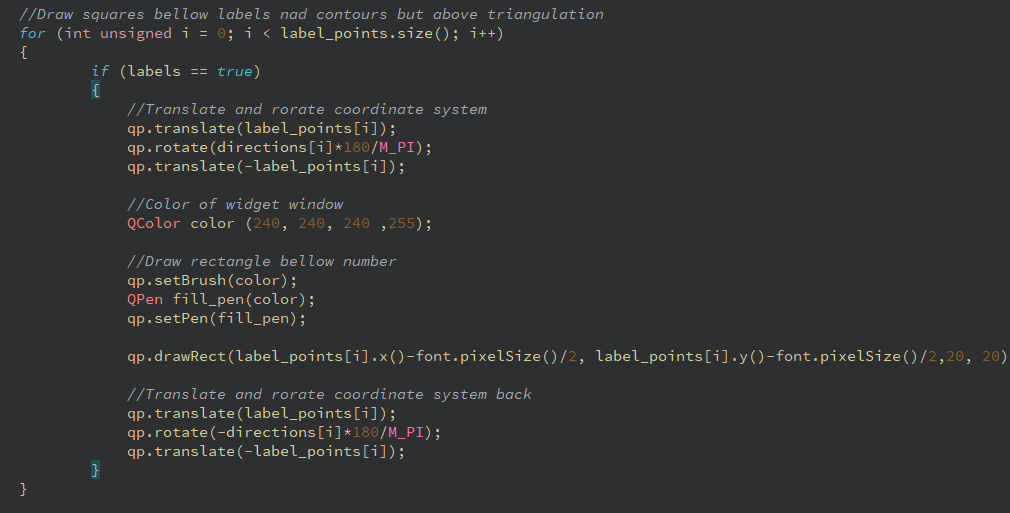
\includegraphics[scale=0.5]{images/DrawLabelSquares.png} 
	\caption{Vykreslování popisů vrstevnic}
	\label{fig:DrawLabels}
\end{figure}

V kódu byla snaha i o otáčení popisů vrstevnic tak, aby bylo možné je číst po směru spádu. Záměr byl takový, že se pro každý segment vrstevnice vypočte směrnice. Dále se vypočtou souřadnice bodu, kde chceme vykreslovat popis vrstevnice ($label_point$. Následně se funkcí getNearestPoint() vypočte nejbližší bod $qn$ ze vstupní množiny bodů $P$ ke zjištěnému $label_point$. Dále se vypočte směrnice přímky mezi $qn$ a $label_point$ a vypočte se výškový rozdíl $dz$ těchto bodů.
Následně se na základě rozdílu vypočtených směrnic a výškového rozdílu $dz$ otočí orientace  popisu vrstevnic o 180 stupňů.

Bohužel, jeli úvaha správná, nepodařilo se nám ji do funkce Algorithms::calculateLabelPoints() zaimplementovat.

\begin{figure}[htbh]
	\centering
	\captionsetup{justification=centering}
	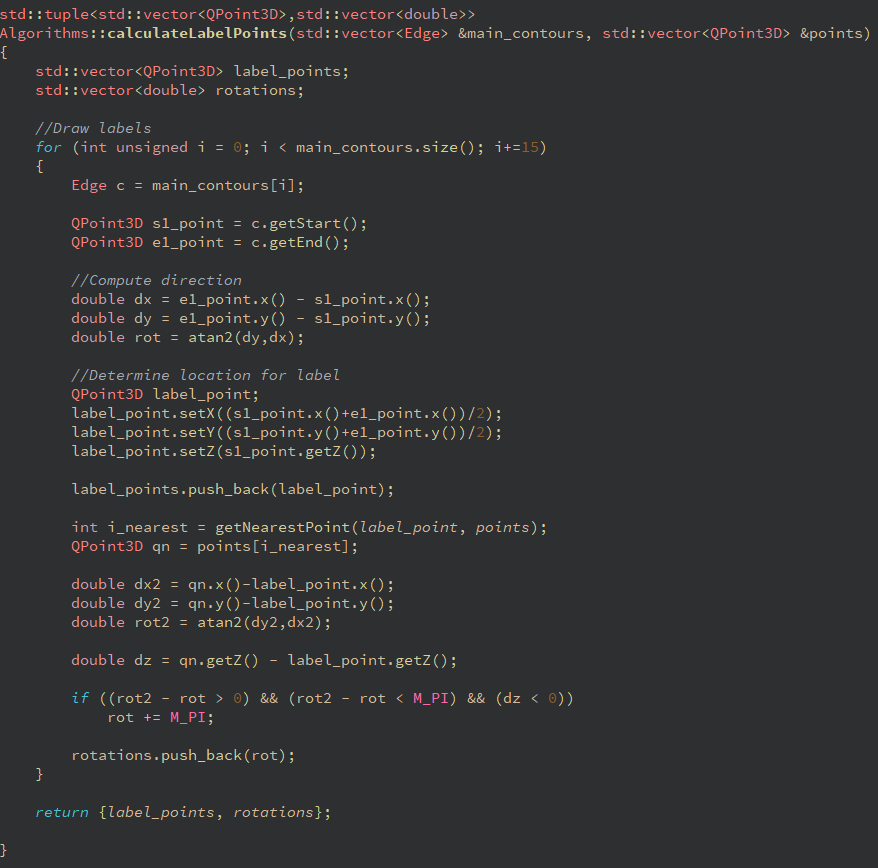
\includegraphics[scale=0.5]{images/code_calculateLabelPoints.png} 
	\caption{Funkce calculateLabelPoints() pro změnu orientace textu podle kartografických zásad}
	\label{fig:code_calculateLabelPoints}
\end{figure}

\clearpage

%----------------------------------------------------------------------------------------
%	VSTUPNÍ DATA
%----------------------------------------------------------------------------------------


\section{Vstupní data}
\subsection{Načítání bodů}

Pro účel aplikace se použila lidarová data DMR 5G. Jelikož byla surová data příliš hustá, byla využita filtrace, která vzala každý desátý bod měření. 

Soubor bodů se souřadnicemi x, y, z se do projektu nahrávají po stisknutí  tlačítka \textit{Load points}. Souřadnice x, y jsou v  souřadnicovém systému S-JTSK a souřadnice z je ve výškovém systému Bpv.

Body jsou načítány postupně řádek po řádku, přičemž musí v nahrávaném souboru platit následující pravidla:    

\begin{itemize}
\item na řádku je pořadí proměnných id >> y (S-JTSK) >> x (S-JTSK)  >> z (Bpv),  hodnoty jsou od sebe odděleny  jednou mezerou,
\item id je identifikátor jednotlivých vrcholů polygonu, x, y, z jsou prostorové souřadnice bodů

\end{itemize}

\begin{figure}[htbh]
	\centering	
	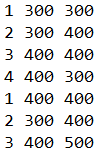
\includegraphics[scale=1]{images/vstup.png} 
	\caption{Špagetový model vstupního souboru bodů}
	\label{fig:vstup.}
\end{figure} 

\subsection{Načítání polygonu}
Polygon, nad kterým lze následně zobrazit triangulaci, se načítá stisknutím tlačítka \textit{Load polygon}.

Každý bod polygonu má ID a rovinné souřadnice x,y v souřadnicovém systému S-JTSK.

Body jsou načítány postupně řádek po řádku, přičemž musí v nahrávaném souboru platit následující pravidla:    

\begin{itemize}
\item na řádku je pořadí proměnných id >> y (S-JTSK) >> x (S-JTSK)  hodnoty jsou od sebe odděleny  jednou mezerou,
\item id je identifikátor jednotlivých vrcholů polygonu, x, y jsou rovinné souřadnice bodů v S-JTSK
\end{itemize}

\begin{figure}[htbh]
	\centering	
	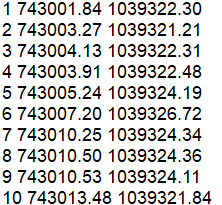
\includegraphics[scale=0.9]{images/vstup_polygon.png} 
	\caption{Špagetový model vstupního souboru polygonu}	\label{fig:vstup_polygon}
\end{figure} 

%----------------------------------------------------------------------------------------
%	VÝSTUPNÍ DATA
%----------------------------------------------------------------------------------------
\section{Výstupní data}
\begin{figure}[htbh]
	\centering
	\captionsetup{justification=centering}
	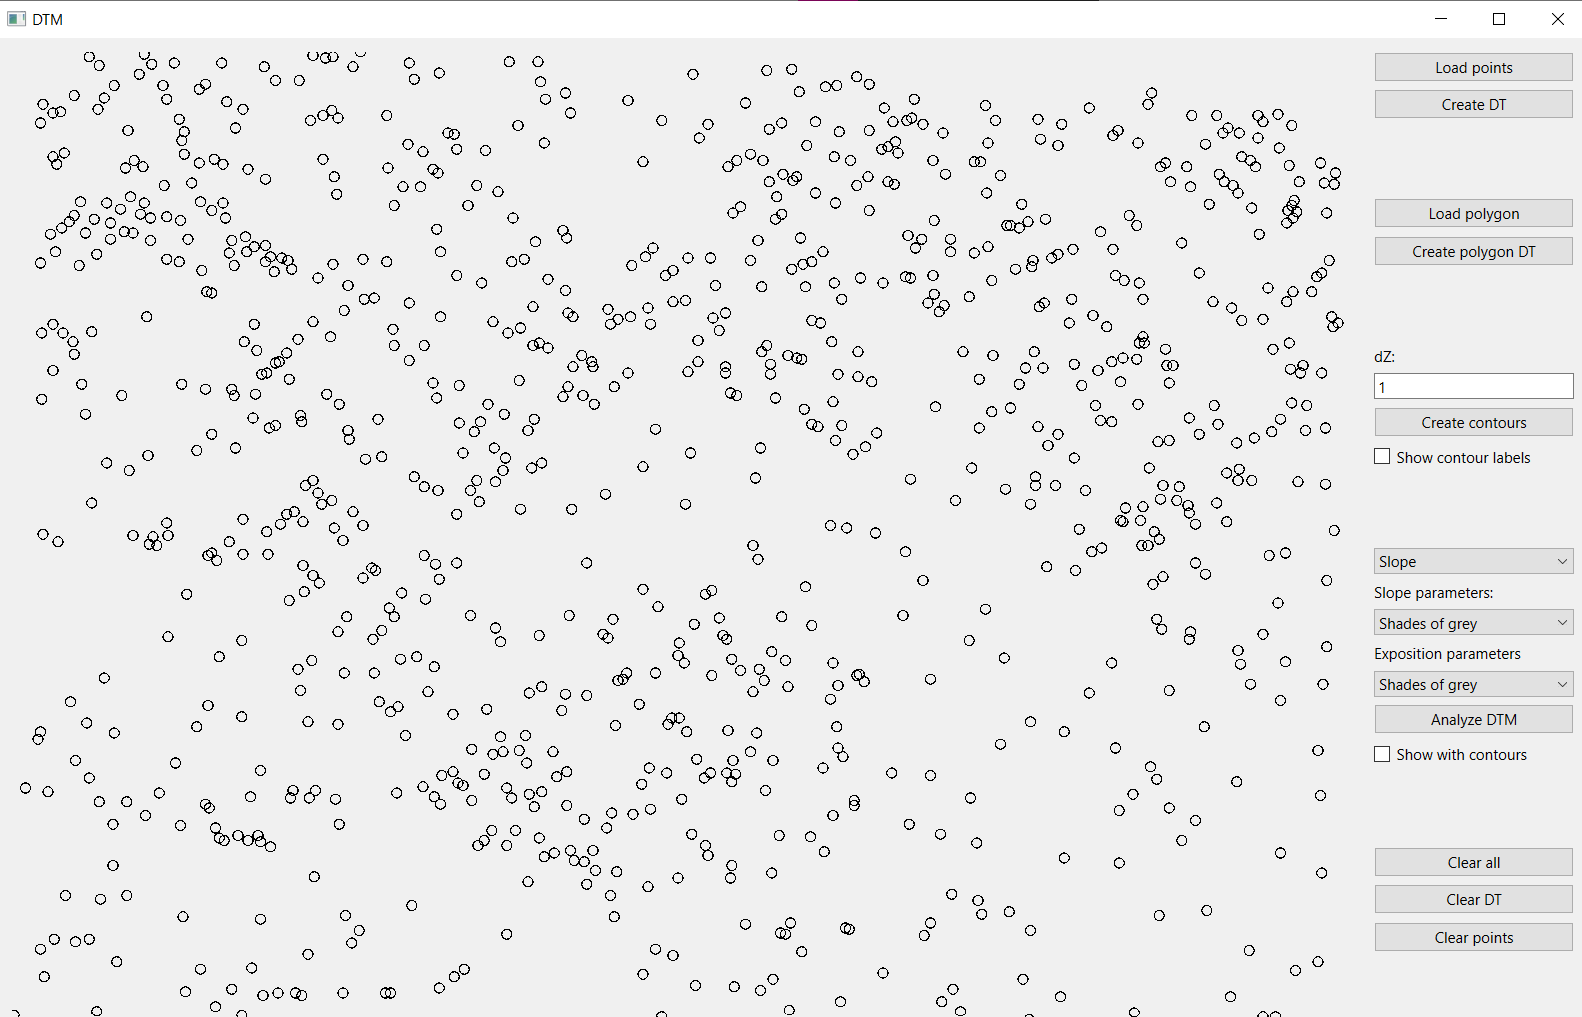
\includegraphics[scale=0.35]{images/vystup_LoadPoints.png} 
	\caption{Aplikace po načtení bodů z textového souboru}
	\label{fig:vystup_LoadPoints}
\end{figure} 
\begin{figure}[htbh]
	\centering
	\captionsetup{justification=centering}
	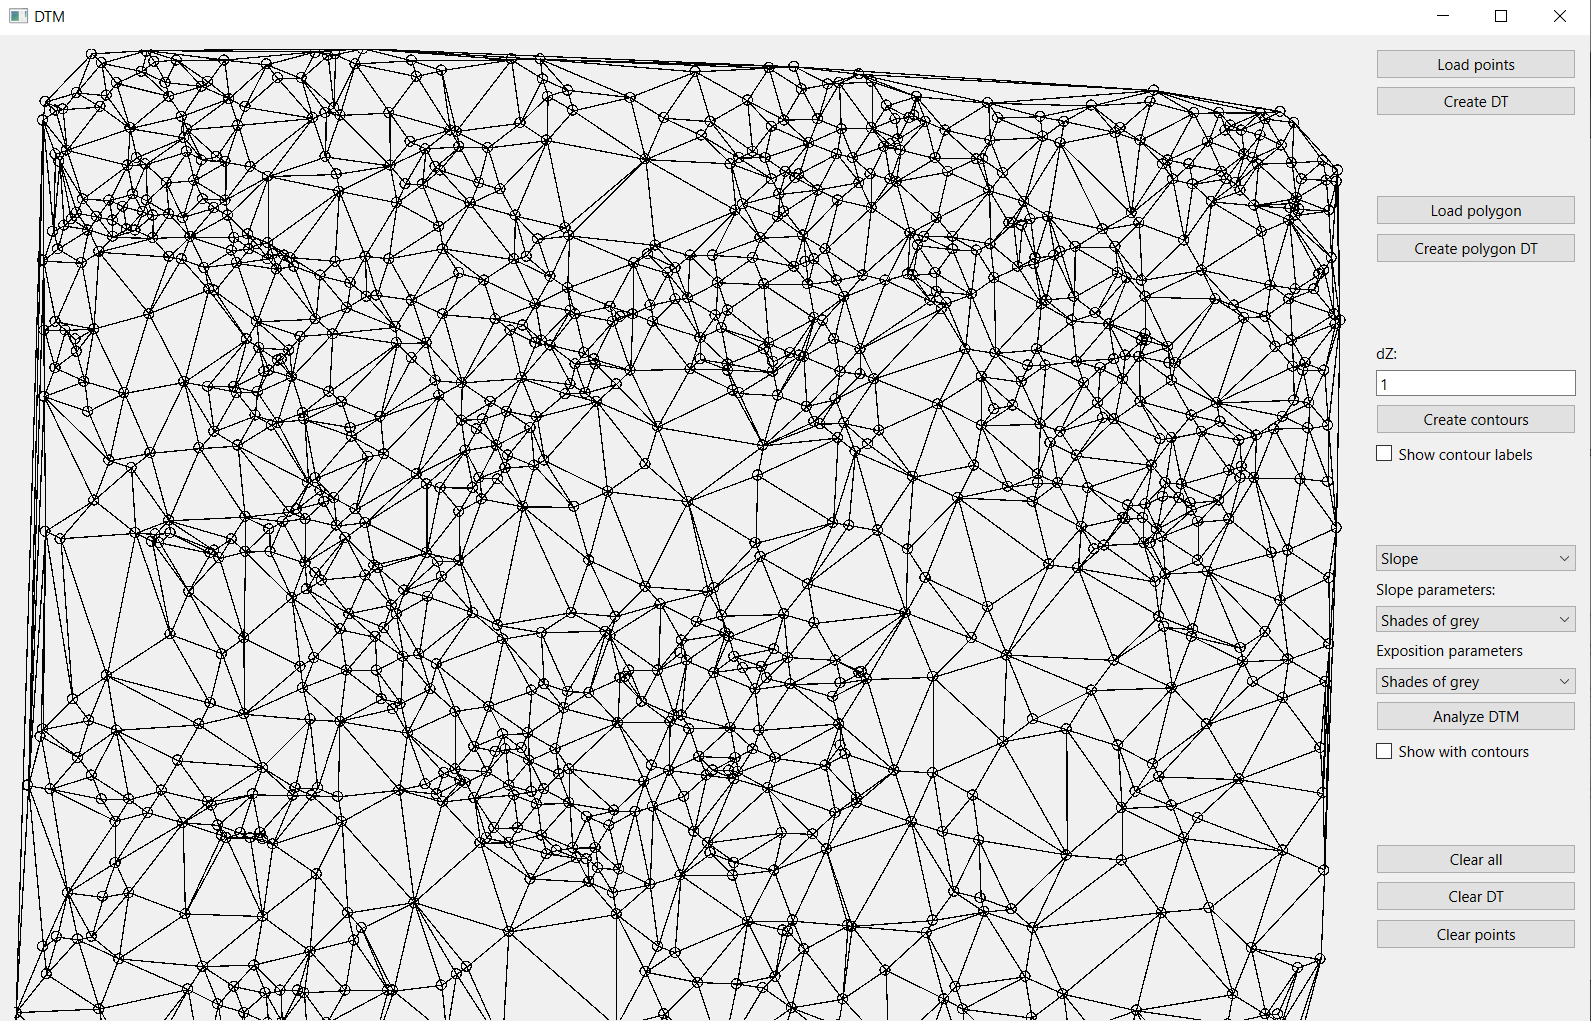
\includegraphics[scale=0.35]{images/vystup_CreateDT.png} 
	\caption{Aplikace po vytvoření Delaunayho triangulace nad množinou bodů}
	\label{fig:vystup_CreateDT}
\end{figure} 
\begin{figure}[htbh]
	\centering
	\captionsetup{justification=centering}
	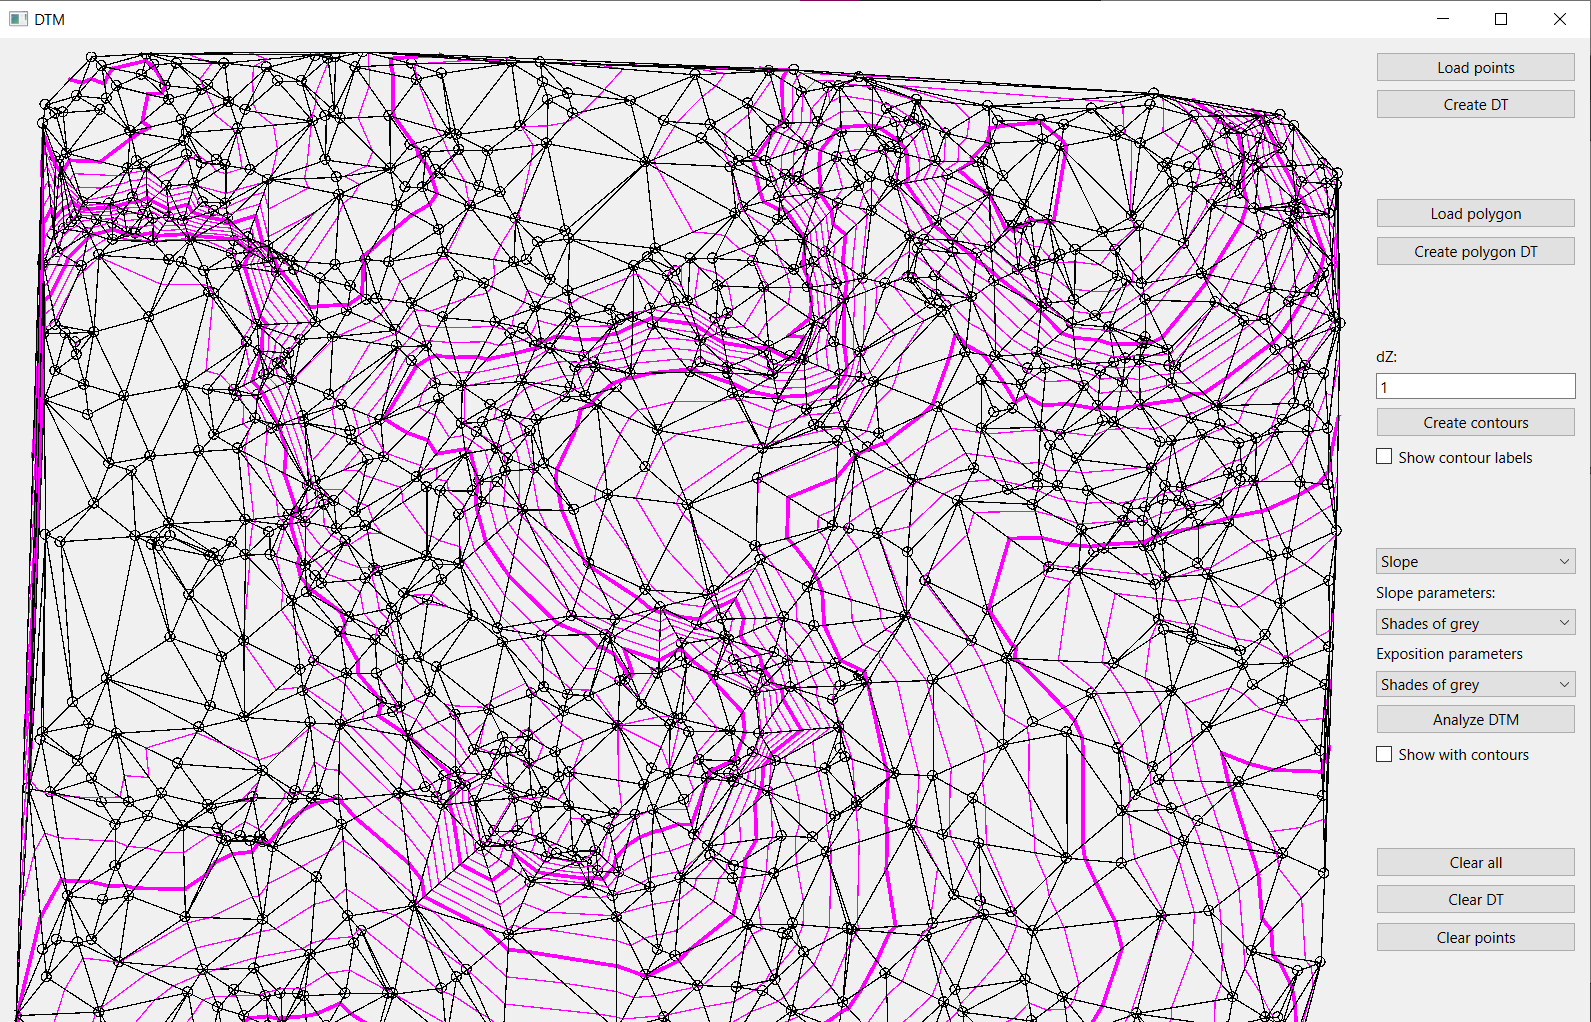
\includegraphics[scale=0.35]{images/vystup_CreateContours.png} 
	\caption{Aplikace po vykreslení vrstevnic}	\label{fig:vystup_CreateContours}
\end{figure} 
\begin{figure}[htbh]
	\centering
	\captionsetup{justification=centering}
	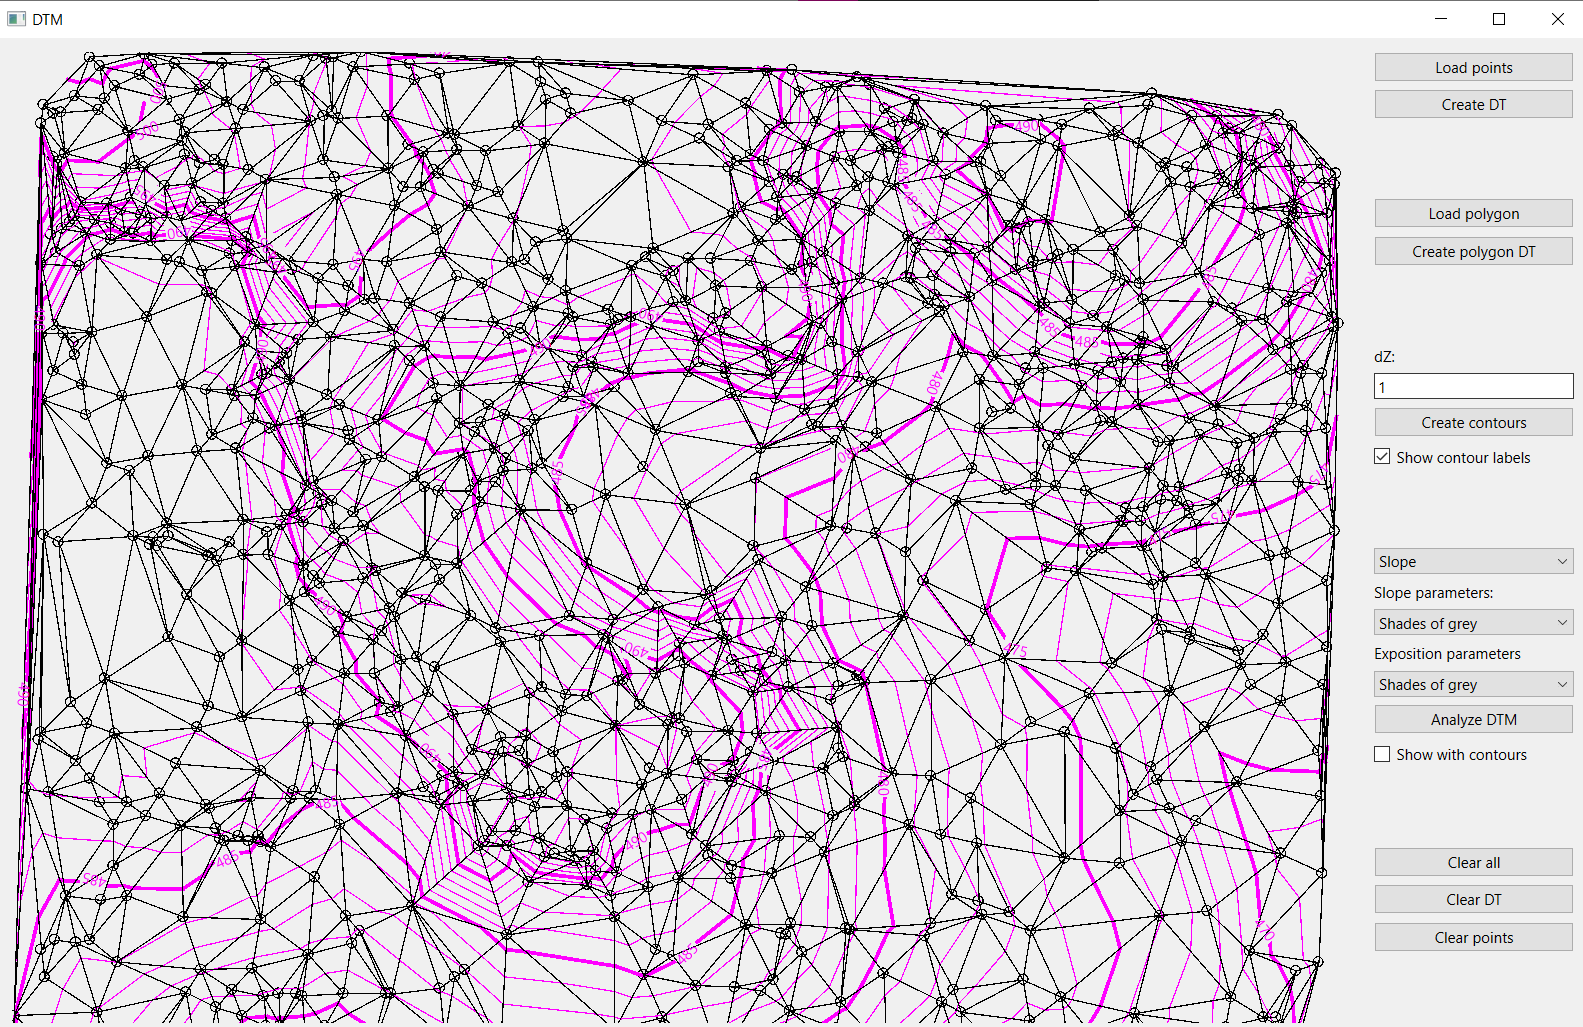
\includegraphics[scale=0.35]{images/vystup_CreateContourswLabels.png} 
	\caption{Aplikace po vykreslení popisů vrstevnic}	\label{fig:vystup_CreateContourssLabels}
\end{figure} 
\begin{figure}[htbh]
	\centering
	\captionsetup{justification=centering}
	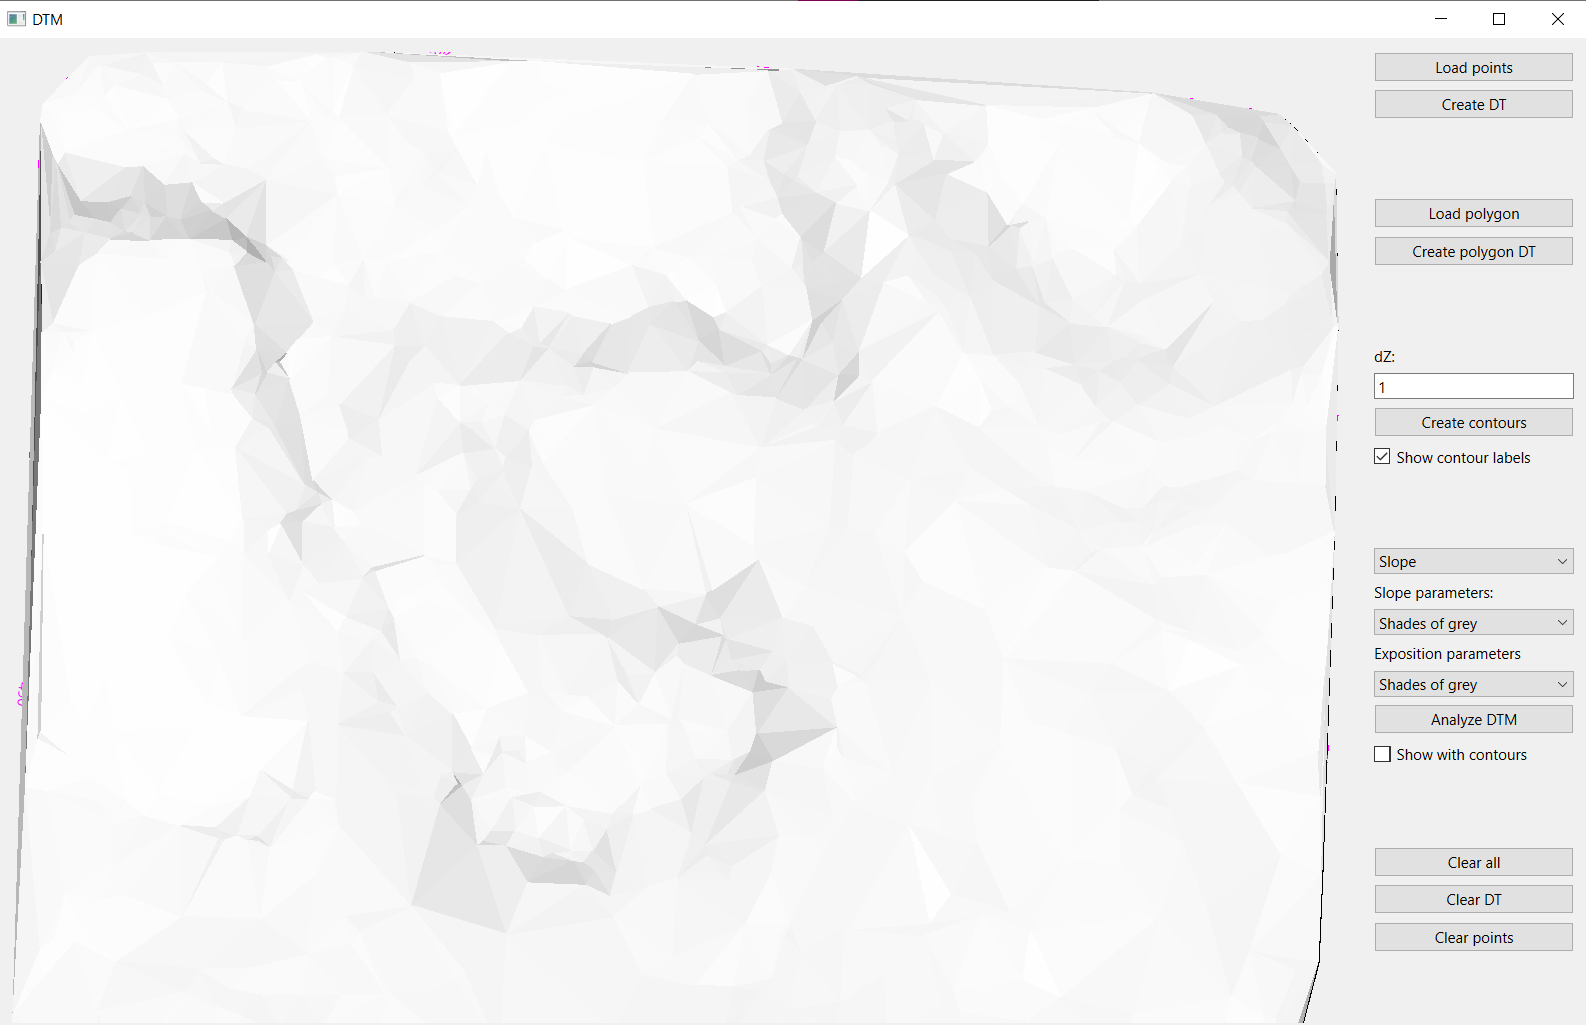
\includegraphics[scale=0.35]{images/vystup_AnalyzeDTM_slope_shadesofgray.png} 
	\caption{Aplikace po vykreslení sklonu terénu v odstínech šedi}	\label{fig:vystup_AnalyzeDTM_slope_shadesofgray}
\end{figure} 
\begin{figure}[htbh]
	\centering
	\captionsetup{justification=centering}
	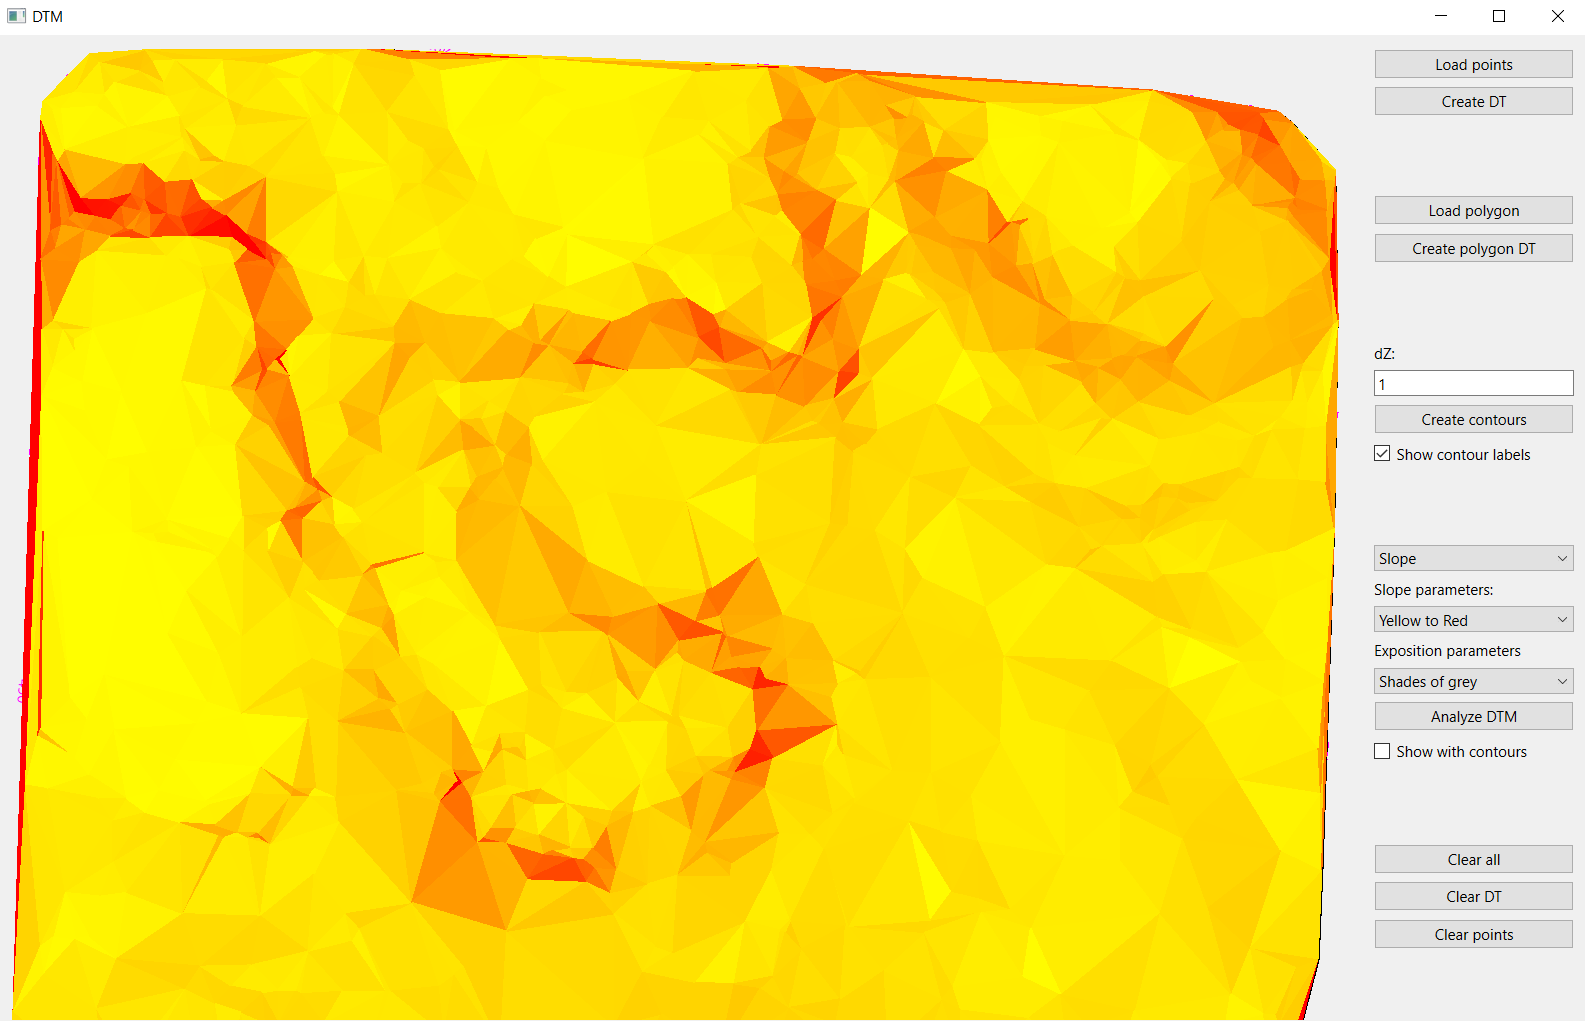
\includegraphics[scale=0.35]{images/vystup_AnalyzeDTM_slope_y2r.png} 
	\caption{Aplikace po vykreslení sklonu terénu v odstínech od žluté po červenou}	\label{fig:vystup_AnalyzeDTM_slope_y2r}
\end{figure} 
\begin{figure}[htbh]
	\centering
	\captionsetup{justification=centering}
	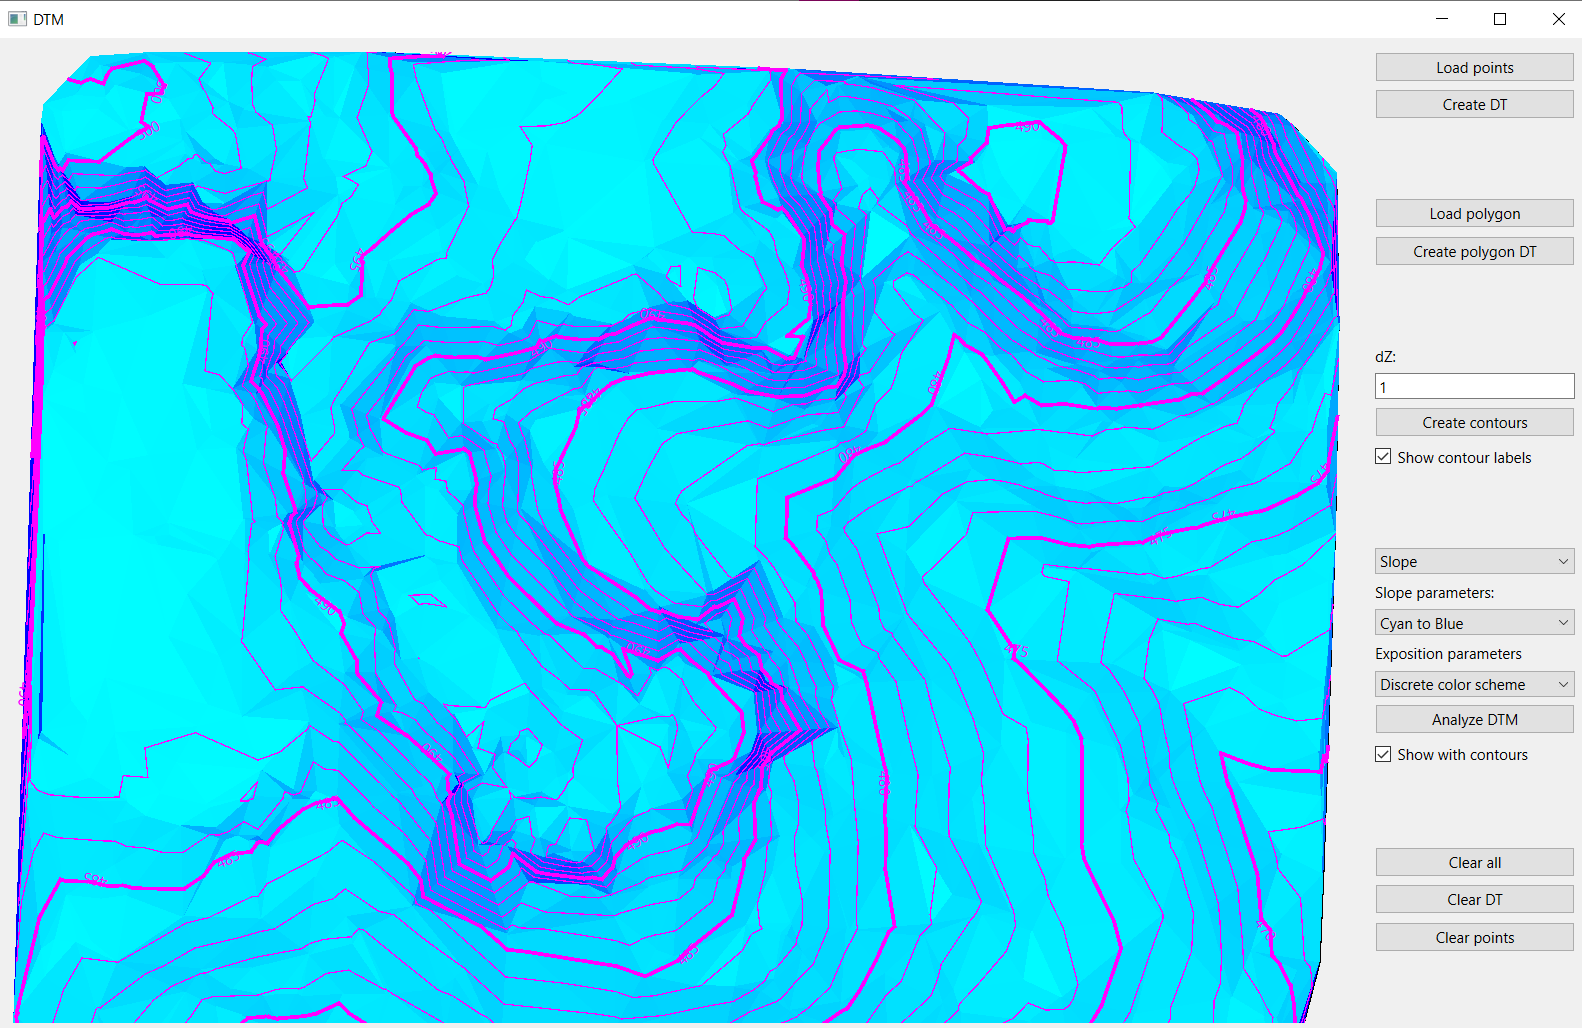
\includegraphics[scale=0.35]{images/vystup_AnalyzeDTM_slope_c2b_wContours.png} 
	\caption{Aplikace po vykreslení sklonu terénu v odstínech od tyrkysové po modrou s vrstevnicemi a popisy vrstevnic}	
\label{fig:vystup_AnalyzeDTM_slope_c2b_wContours}
\end{figure}
\begin{figure}[htbh]
	\centering
	\captionsetup{justification=centering}
	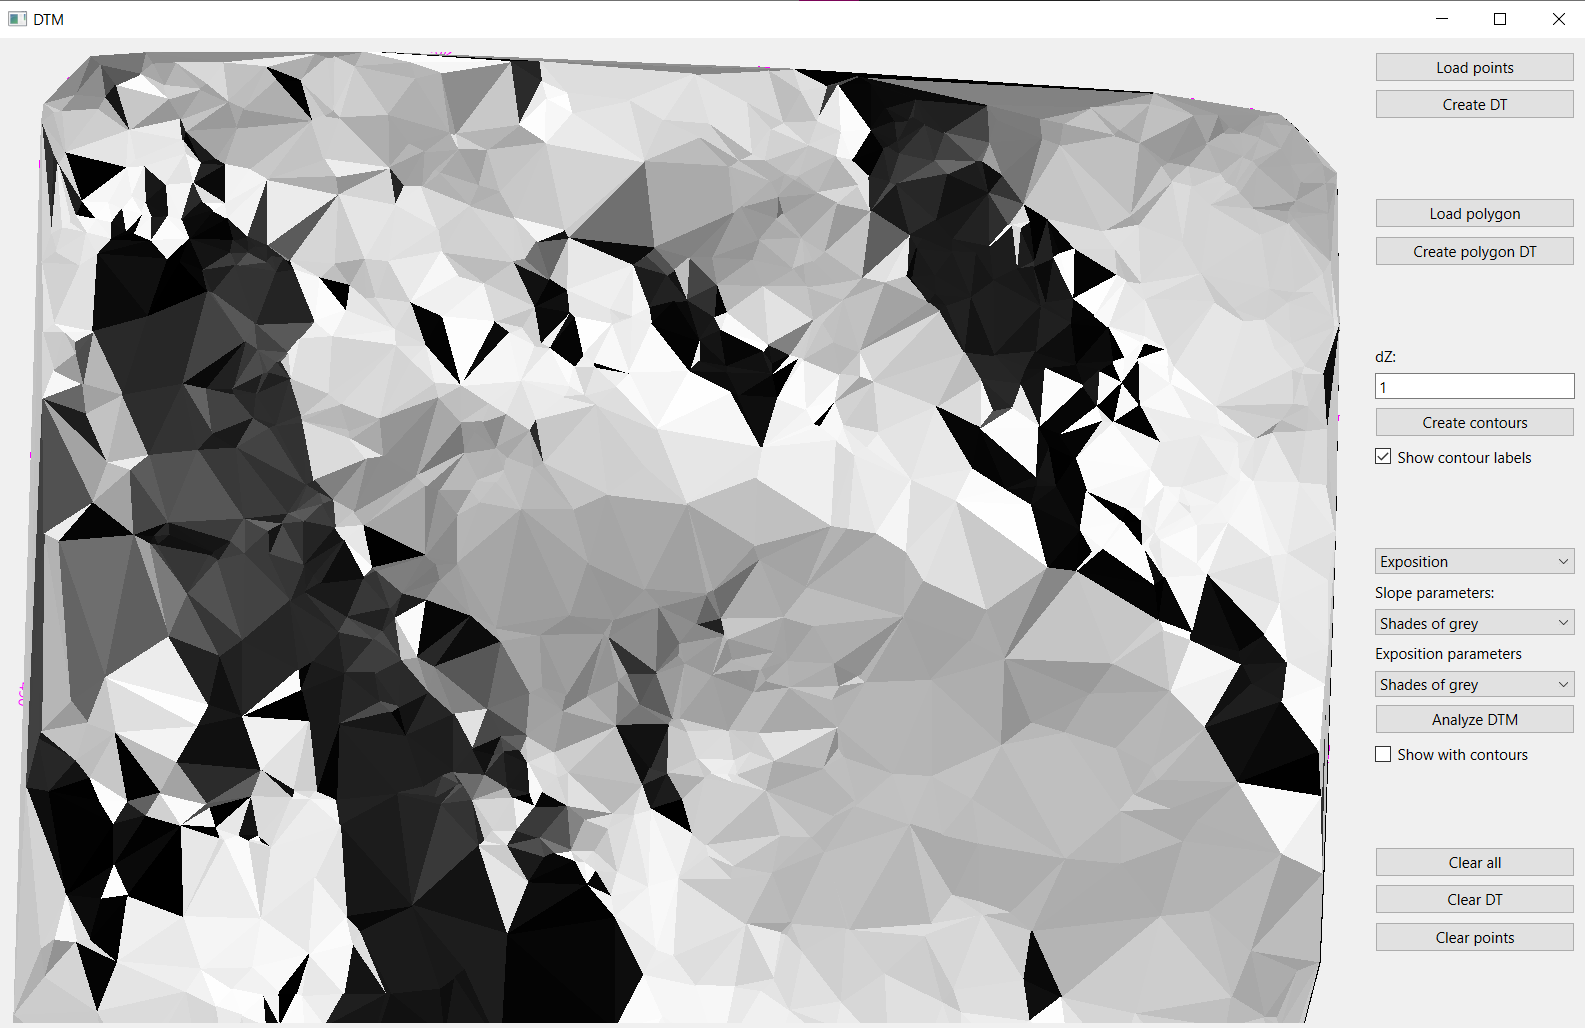
\includegraphics[scale=0.35]{images/vystup_AnalyzeDTM_exposition_shadesofgrey.png} 
	\caption{Aplikace po vykreslení expozice terénu v odstínech šedi}	\label{fig:vystup_AnalyzeDTM_exposition_shadesofgrey}
\end{figure} 
\begin{figure}[htbh]
	\centering
	\captionsetup{justification=centering}
	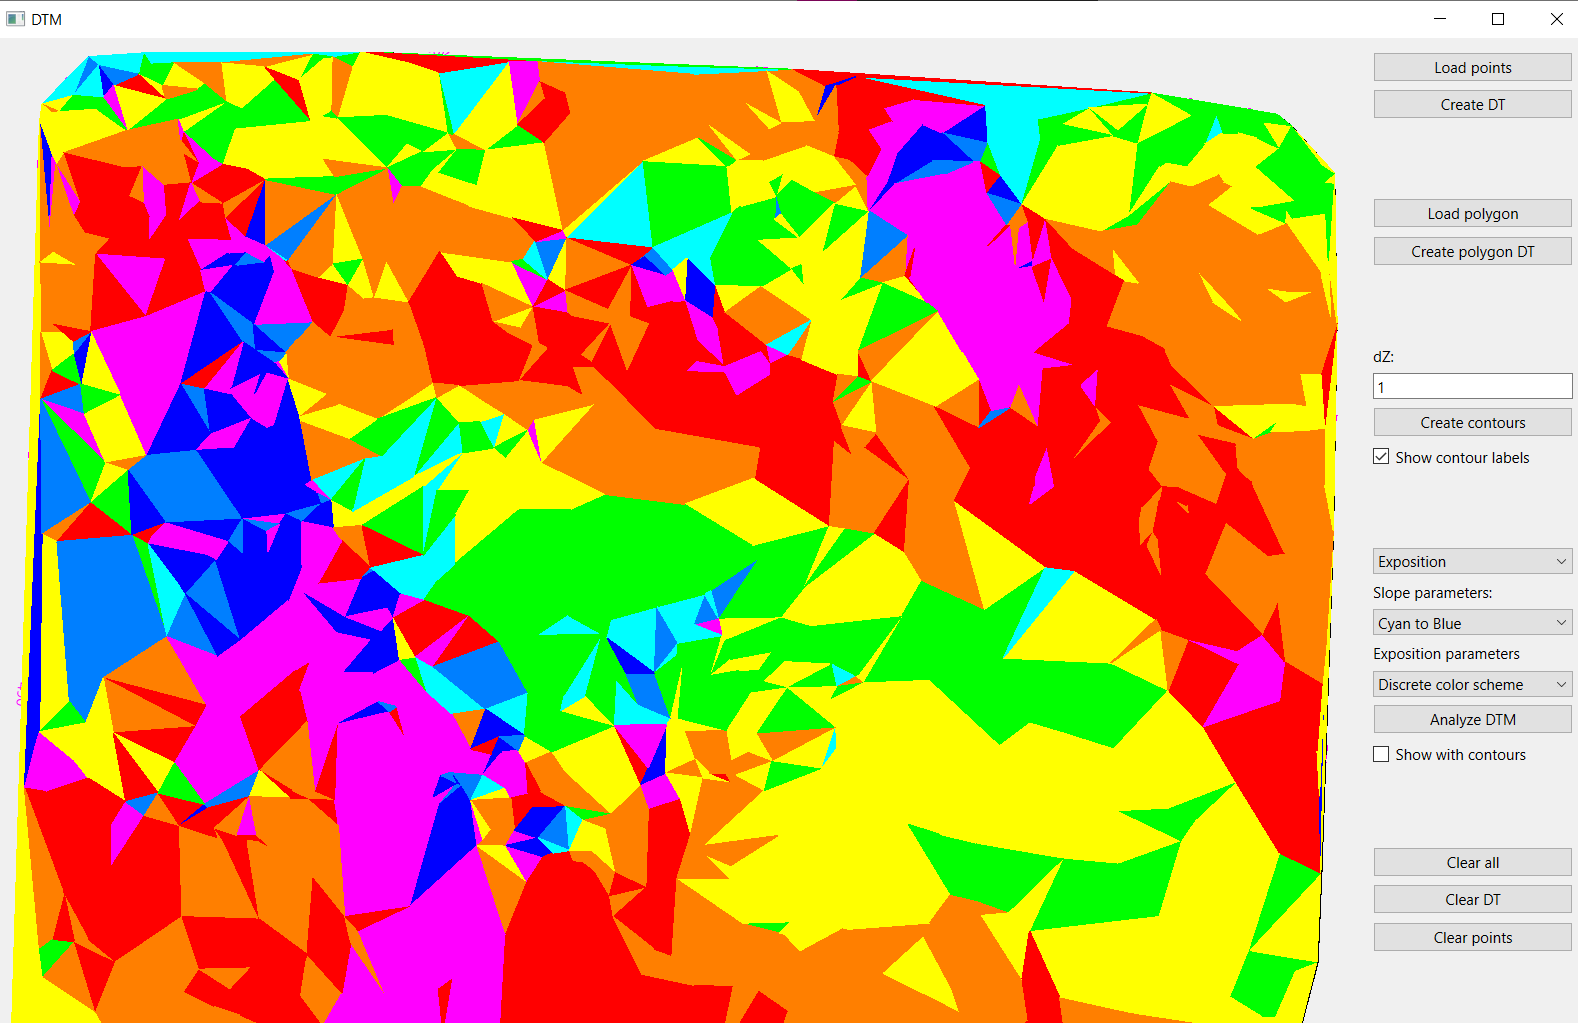
\includegraphics[scale=0.35]{images/vystup_AnalyzeDTM_exposition_discrete.png} 
	\caption{Aplikace po vykreslení expozice terénu v barvách podle tříd z obrázku \ref{fig:getExposition()}}	\label{fig:vystup_AnalyzeDTM_exposition_discrete}
\end{figure} 
\begin{figure}[htbh]
	\centering
	\captionsetup{justification=centering}
	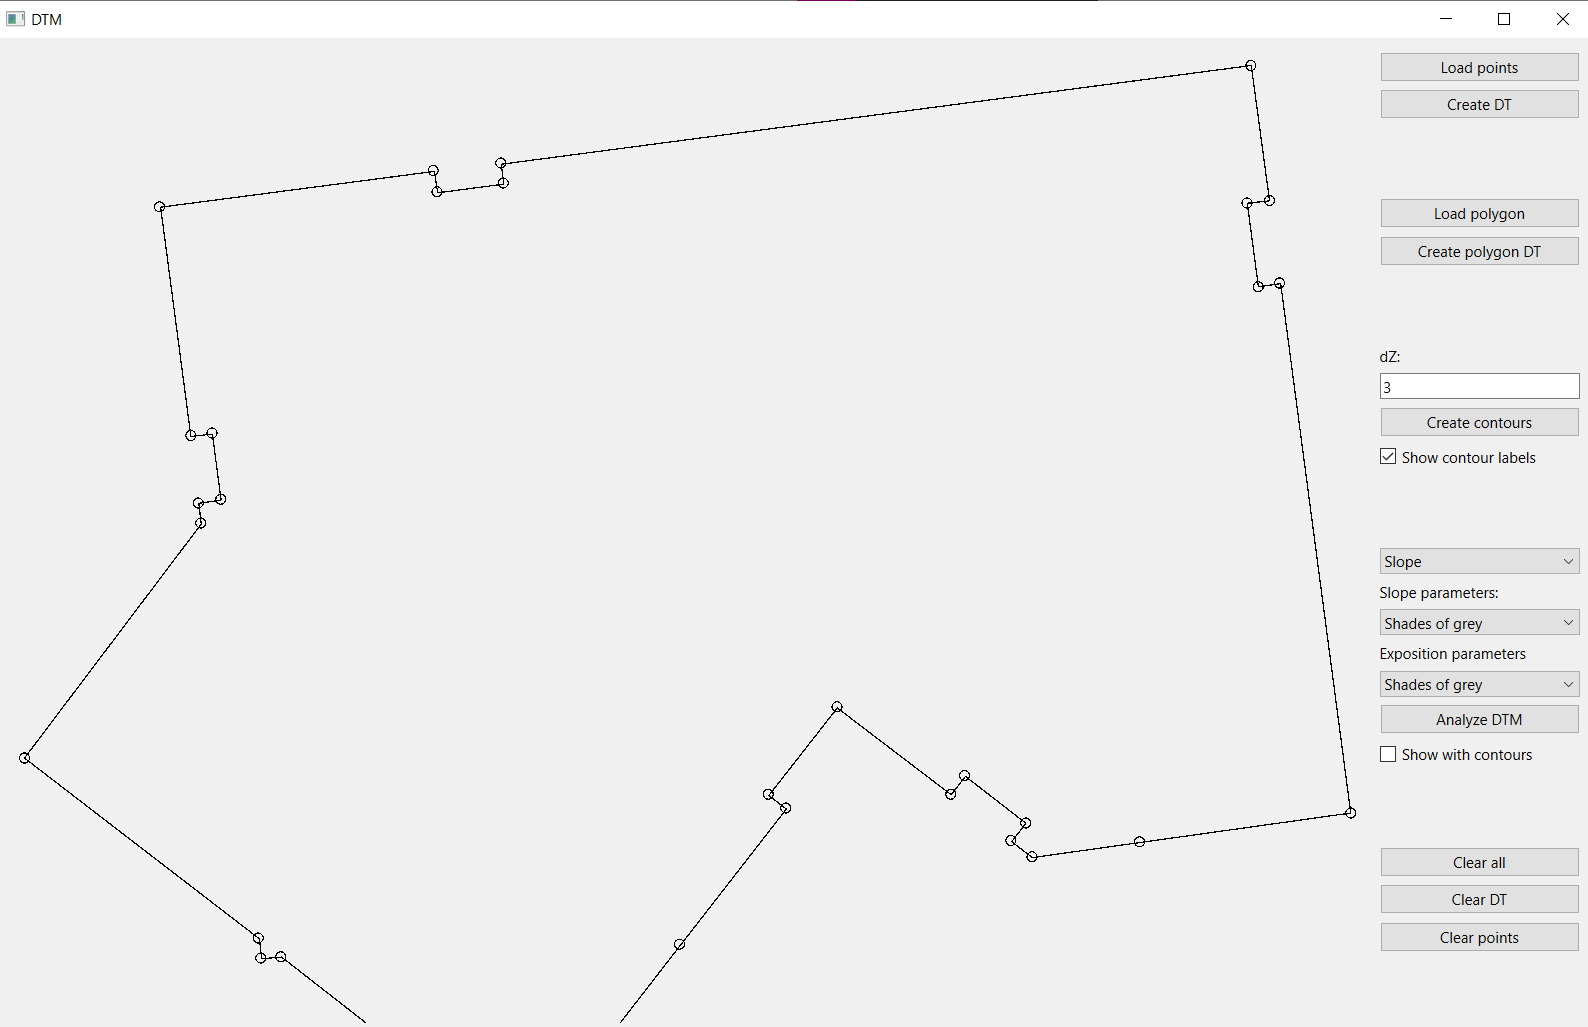
\includegraphics[scale=0.35]{images/vystup_LoadPolygon.png} 
	\caption{Aplikace po načtení polygonu z textového souboru}	\label{fig:vystup_LoadPolygon}
\end{figure} 
\begin{figure}[htbh]
	\centering
	\captionsetup{justification=centering}
	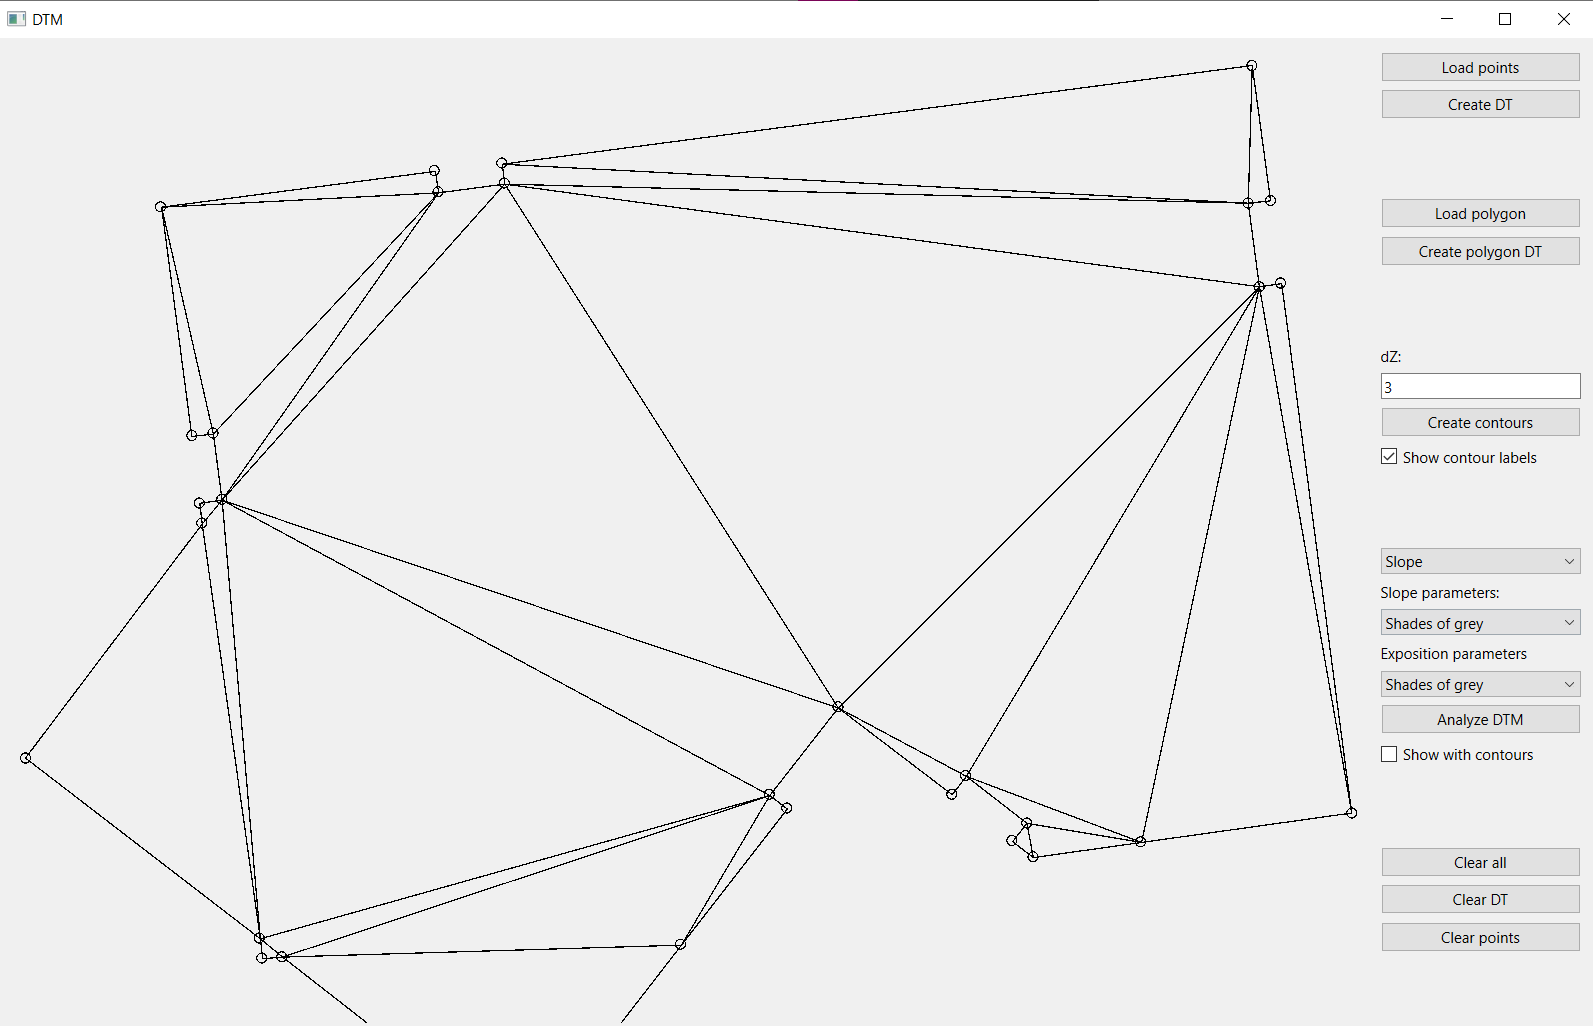
\includegraphics[scale=0.35]{images/vystup_CreateDT_pol.png} 
	\caption{Aplikace po vytvoření Delaunayho triangulace nad nekonvexním polygonem}
	\label{fig:vystup_CreateDT_pol}
\end{figure} 
\begin{figure}[htbh]
	\centering
	\captionsetup{justification=centering}
	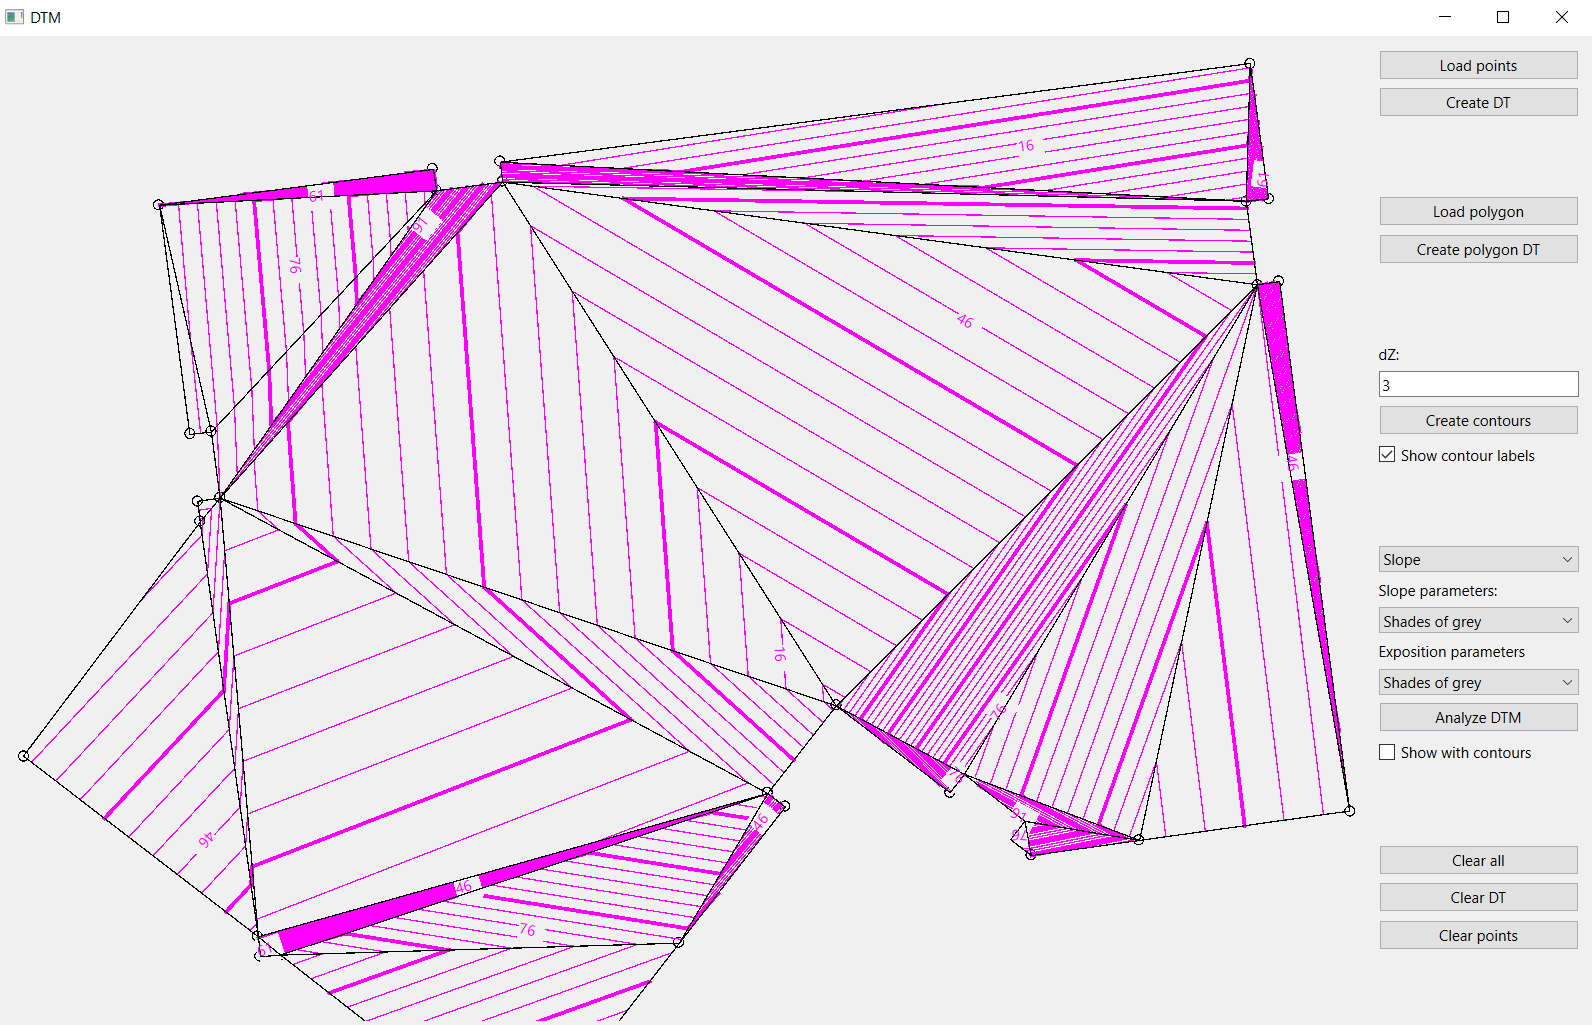
\includegraphics[scale=0.35]{images/vystup_CreateContourswLabels_pol.png} 
	\caption{Aplikace po vykreslení vrstevnic s popisy nad DT nekonvexního polygonu}	\label{fig:vystup_CreateContourssLabels_pol}
\end{figure} 
\begin{figure}[htbh]
	\centering
	\captionsetup{justification=centering}
	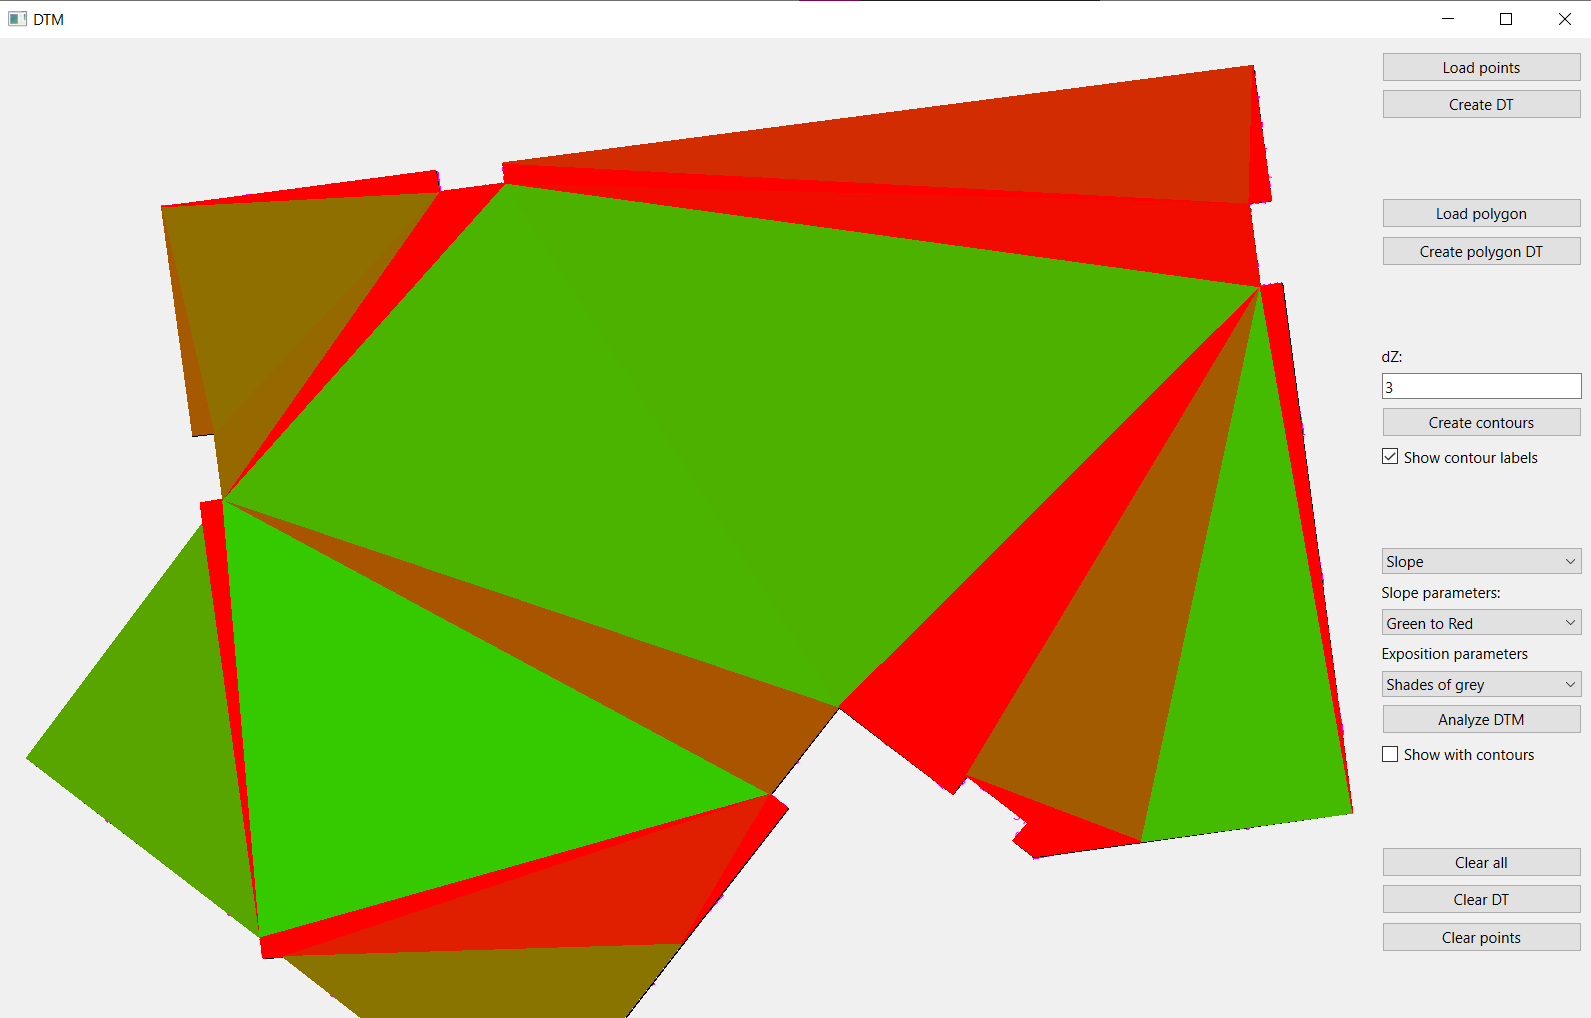
\includegraphics[scale=0.35]{images/vystup_AnalyzeDTM_slope_g2r_pol.png} 
	\caption{Aplikace po vykreslení sklonu terénu nad nekonvexním polygonem v odstínech od zelené po červenou}	\label{fig:vystup_AnalyzeDTM_slope_g2r_pol}
\end{figure} 
\begin{figure}[htbh]
	\centering
	\captionsetup{justification=centering}
	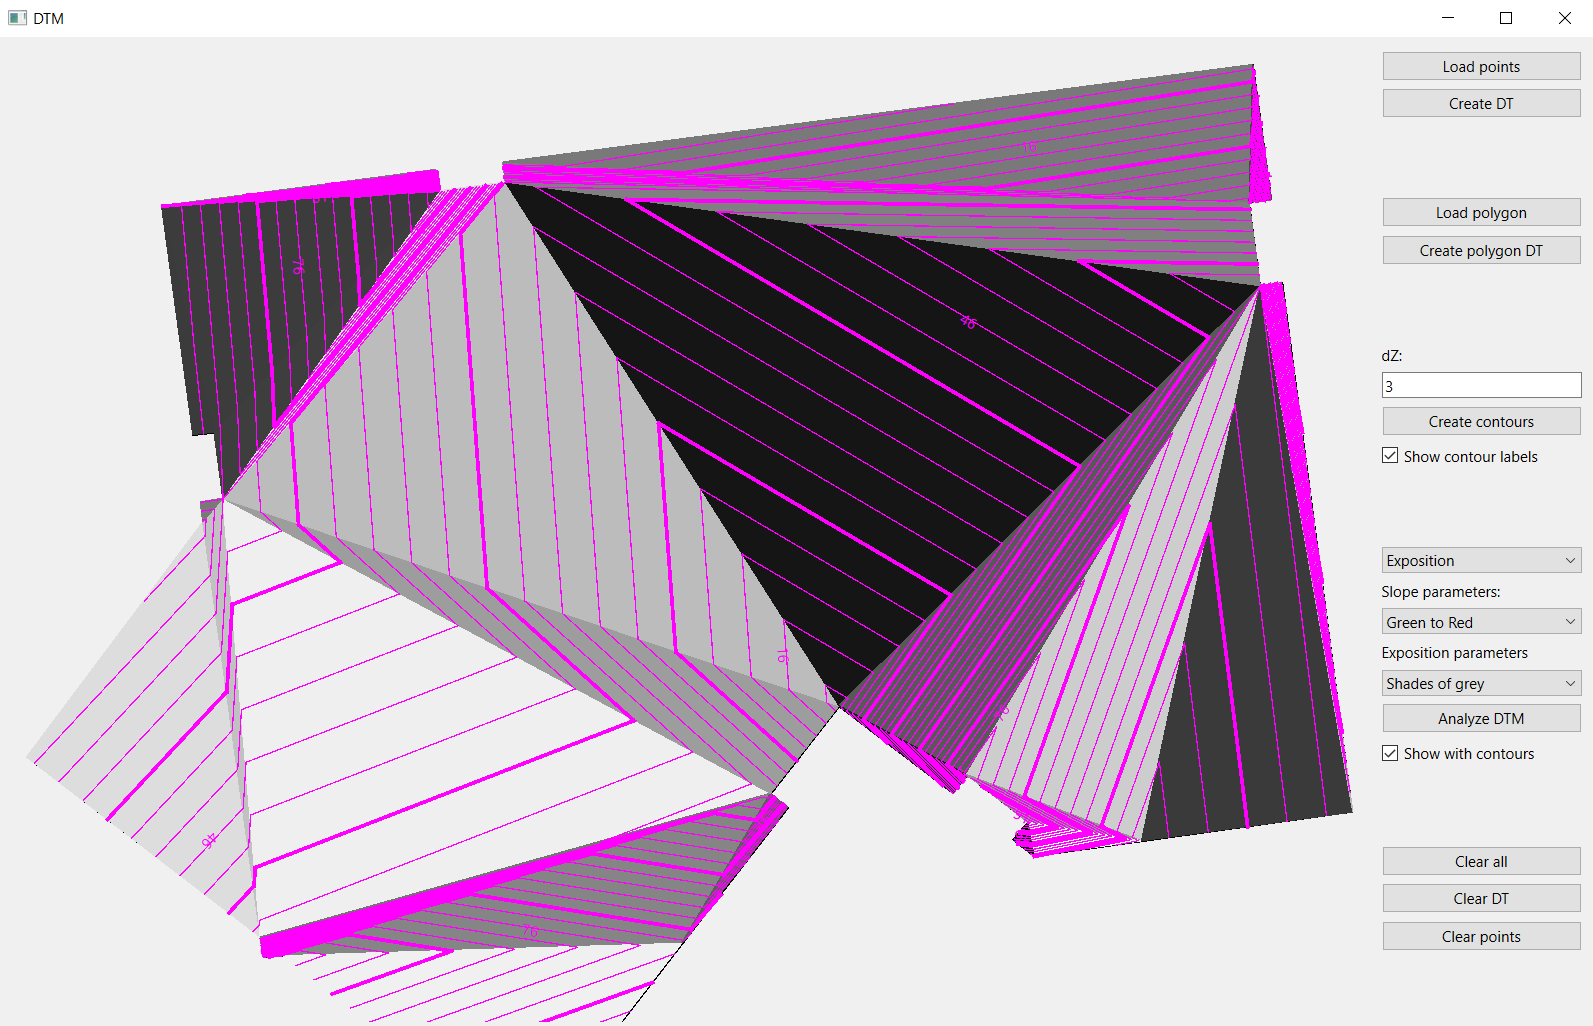
\includegraphics[scale=0.35]{images/vystup_AnalyzeDTM_exposition_shadesofgrey_pol_wContours.png} 
	\caption{Aplikace po vykreslení expozice nekonvexního polygonu v odstínech šedi s vykreslenými vrstevnicemi a jejich popisy}	\label{fig:vystup_AnalyzeDTM_exposition_shadesofgrey_pol_wContours}
\end{figure} 
\begin{figure}[htbh]
	\centering
	\captionsetup{justification=centering}
	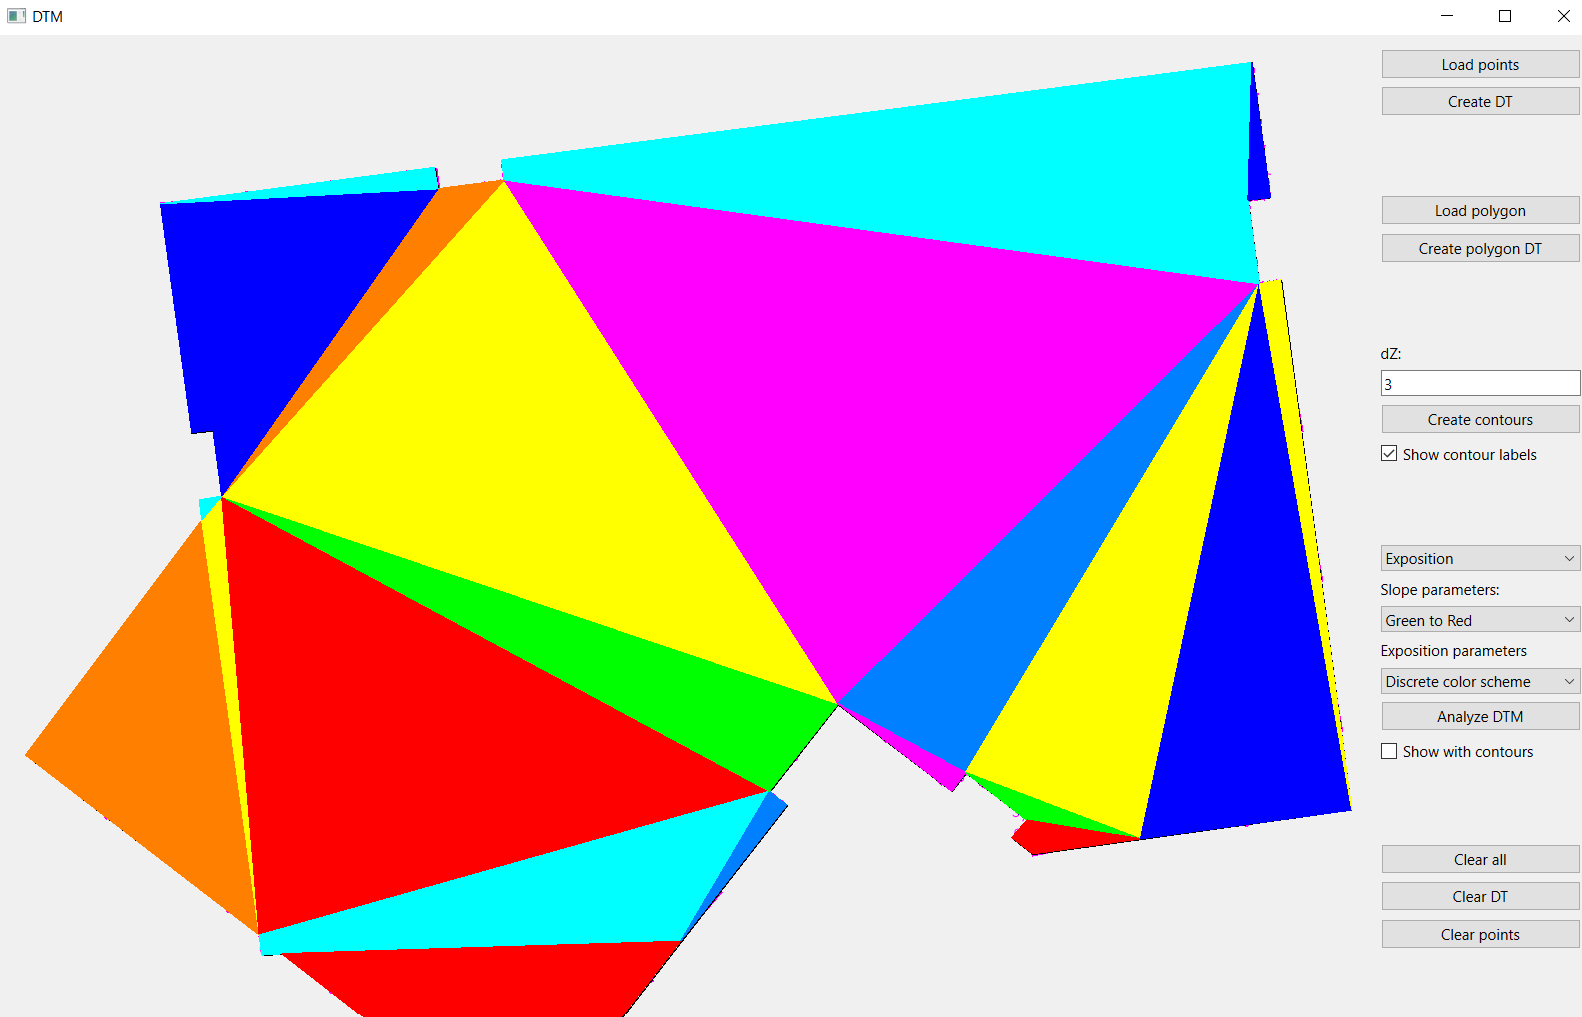
\includegraphics[scale=0.35]{images/vystup_AnalyzeDTM_exposition_discrete_pol.png} 
	\caption{Aplikace po vykreslení expozice nekonvexního polygonu v barvách podle tříd z obrázku \ref{fig:getExposition()}}	\label{fig:vystup_AnalyzeDTM_exposition_discrete_pol}
\end{figure} 
\clearpage

\section{Printscreen vytvořené aplikace}
\begin{figure}[htbh]
	\centering
	
	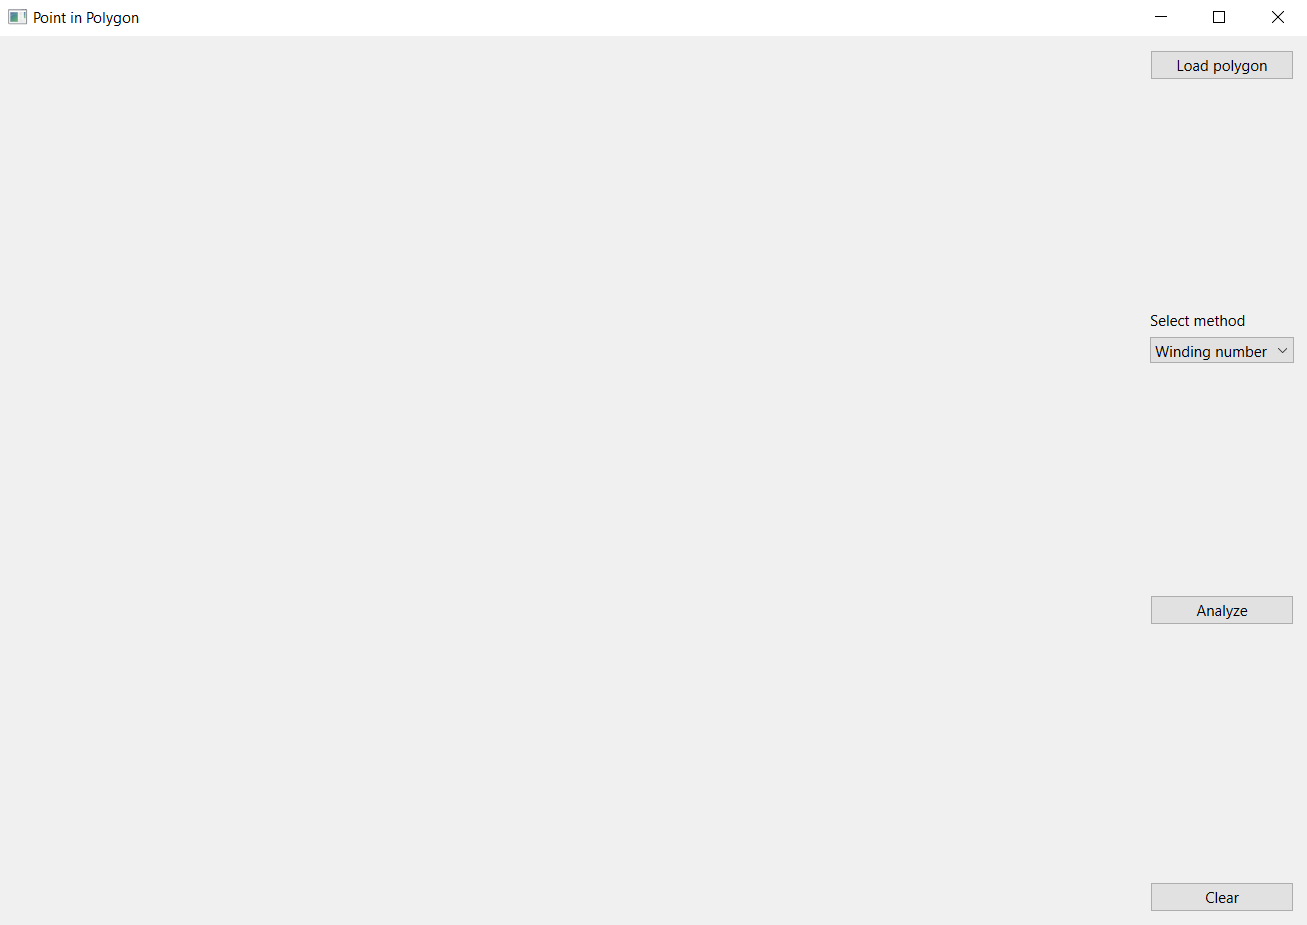
\includegraphics[scale=0.4]{images/aplikace_uvodni_okno.png} 
	\caption{Úvodní okno aplikace}
	\label{fig:uvodni_okno}
\end{figure} 

\clearpage

%----------------------------------------------------------------------------------------
%	DOKUMENTACE
%----------------------------------------------------------------------------------------

\section{Dokumentace}
Kód zahrnuje 3 třídy – Draw, Algorithms a Widget, které budou následně detailněji popsány.      

\subsection{Třída Algorithms}
Třída Algorithms obsahuje 14 funkcí:  

\begin{itemize}
	\item 0 v případě, že bod leží v pravé polorovině,
	\item 1 v případě, že  bod leží v levé polorovině,
	\item -1 v případě, že bod leží na linii.
\end{itemize}

\begin{itemize}
	\item double get2LinesAngle(QPoint \&p1, QPoint \&p2, QPoint \&p3, QPoint \&p4);
	\item std::tuple<QPoint3D,double> getCircleCenterAndRadius(QPoint3D \&p1,QPoint3D \&p2,QPoint3D \&p3);
	\item int getDelaunayPoint(QPoint3D \&s,QPoint3D \&e,std::vector<QPoint3D> \&points);
	\item int getNearestPoint(QPoint3D \&p, std::vector<QPoint3D> \&points);
	\item std::vector<Edge> dT(std::vector<QPoint3D> \&points);
	\item std::vector<Edge> dTPolygon(std::vector<QPoint3D> \&points);
	\item void updateAEL(Edge \&e, std::list<Edge> \&ael);
	\item QPoint3D getContourPoint(QPoint3D \&p1, QPoint3D \&p2, double z);
	\item std::vector<Edge> getContourLines(std::vector<Edge> \&dt, double zmin, double zmax, double dz);
	\item double getSlope(QPoint3D \&p1, QPoint3D \&p2, QPoint3D \&p3);
	\item double getExposition(QPoint3D \&p1, QPoint3D \&p2, QPoint3D \&p3);
	\item std::vector<Triangle> analyzeDTM(std::vector<Edge> \&dt);
	\item QPoint3D getCentreOfMass(QPoint3D \&p1, QPoint3D \&p2, QPoint3D \&p3);
	\item int getPositionWinding(QPoint3D \&q, std::vector<QPoint3D> \&pol);
	\item int getPointLinePosition(QPoint \&a, QPoint \&p1, QPoint \&p2);
\end{itemize}


\paragraph{double get2LinesAngle(QPoint \&p1, QPoint \&p2, QPoint \&p3, QPoint \&p4);}
Počítá úhel mezi dvěma liniemi. Vstupními argumenty jsou body určující linie, tzn. vrcholy polygonu. Návratovou hodnotou funkce je double – desetinné číslo s velikostí úhlu mezi těmito přímkami.  

\paragraph{std::tuple<QPoint3D,double> getCircleCenterAndRadius(QPoint3D \&p1,QPoint3D \&p2,QPoint3D \&p3);}
Funkce počítá poloměr a střed vepsaného trojúhelníku. Vstupními argumenty jsou vrcholy trojúhelníku uložené v datovém typu QPoint3D, výstupním je střed trojúhelníku (QPoitn3D) a hodnota poloměru trojúhelníku (double).

\paragraph {int getDelaunayPoint(QPoint3D \&s,QPoint3D \&e,std::vector<QPoint3D> \&points);}
Funkce hledá Delaunay bod. Vstupními argumenty jsou 2 body Delaunay triangulace a vektor QPoint3D bodů, z nichž je hledán Delaunay bod. Výstupním argumentem funkce je index nalezeného bodu uložený jako integer.

\paragraph {int getNearestPoint(QPoint3D \&p, std::vector<QPoint3D> \&points);}
Fun\-kce vyhledává k zadanému bodu bod nejbližší ze zadané množiny. Vstupním argumentem je bod QPoint3D, k němuž hledáme bod nebližší vektor bodů QPoint3D, výsledným je nejbližší nalezený bod – QPoint3D.

\paragraph{std::vector<Edge> dT(std::vector<QPoint3D> \&points);}
Funkce počítá De\-launay triangulaci. Vstupním argumentem funkce je vektor bodů obsahující souřadnice x, y, z. Výstupním argumentem je vektor hran (Edge) vytvořené 
Delaunay triangulace.

\paragraph {std::vector<Edge> dTPolygon(std::vector<QPoint3D> \&points);}
Funkce počítá Delaunay triangulaci nekonvexního polygonu. Vstupním argumentem funkce je vektor uzlů polygonu obsahující souřadnice x, y, z. Výstupním argumentem je vektor hran (Edge) vytvořené Delaunay triangulace.

\paragraph {void updateAEL(Edge \&e, std::list<Edge> \&ael);}

\paragraph {QPoint3D getContourPoint(QPoint3D \&p1, QPoint3D \&p2, double z);}
Funkce hledá mezi dvěma zadanými body lineární interpolací bod v zadané výšce. Vstupními argumenty jsou 2 body QPoint3D a výška, jejíž hodnotu má výsledná vrstevnice mít. Výstupní hodnotou je nalezený průsečík uložený v datovém typu QPoint3D.

\paragraph {std::vector<Edge> getContourLines(std::vector<Edge> \&dt, double zmin, double zmax, double dz);}
Funkce vytváří vrstevnice o zadaném základním intervalu. Vstupním argumentem je De\-launay triangulace, maximální a minimální hodnota souřadnice z a dz, což je základní interval vrstevnic. Výstupním argumentem je vektor hran s vytvořenými vrstevnicemi.

\paragraph {double getSlope(QPoint3D \&p1, QPoint3D \&p2, QPoint3D \&p3);}
Funkce počítá hodnotu sklonu trojúhelníku Delaunay triangulace. Vstupními argumenty jsou vrcholy trojúhelníku uložené v datovém typu QPoint3D, výstupním je hodnota sklonu.

\paragraph {double getExposition(QPoint3D \&p1, QPoint3D \&p2, QPoint3D \&p3);}
Funkce počítá hodnotu expozice trojúhelníku Delaunay triangulace. Vstupními argumenty jsou vrcholy trojúhelníku uložené v datovém typu QPoint3D, výstupním je hodnota expozice.

\paragraph {std::vector<Triangle> analyzeDTM(std::vector<Edge> \&dt);}
Funkce analyzuje všechny trojúhelníky vytvořené Delaunay triangulací – počítá jejich sklon, expozici. Vstupním argumentem je vektor hran Delaunay triangulace, výstupním je vektor Triangle, v němž jsou uložené hrany jednotlivých trojúhelníků, jejich sklony a expozice.

\paragraph {QPoint3D getCentreOfMass(QPoint3D \&p1, QPoint3D \&p2, QPoint3D \&p3);}
Funkce počítá těžiště trojúhelníku. Vstupními argumenty jsou vrcholy trojúhelníku uložené v datovém typu QPoint3D, výstupním je bod těžiště trojúhelníku v datovém typu QPoint3D. 

\paragraph{int getPositionWinding(QPoint \&q, std::vector<QPoint> \&pol);}\mbox{}\\
Funkce analyzuje polohu bodu metodou Winding Number, jež byla podrobně vysvětlena v kapitole 3.  Vstupními argumenty jsou souřadnice bodu $q$ (jako QPoint) a vektor vrcholů polygonu (vektor naplněný prvky QPoint). Funkce vrací integer, jež může nabývat 3 hodnot:

\begin{itemize}
	\item 1, leží-li analyzovaný bod uvnitř polygonu
	\item -1 leží-li na linii polygonu 
	\item a 0, leží-li mimo kontrolovaný polygon.
\end{itemize}

\paragraph{int getPointLinePosition(QPoint \&a, QPoint \&p1, QPoint \&p2);}
Analyzuje vzájemnou polohu mezi bodem a linií polygonu, resp. v jaké polorovině vůči linii se bod nachází. Vstupními argumenty funkce jsou souřadnice určovaného bodu (jako QPoint) a souřadnice 2 bodů určujících polohu linie (vrcholy polygonu taktéž jako QPoint). Funkce vrací vždy hodnotu 1, 0 nebo -1 dle následujících pravidel:

\begin{itemize}
	\item 0 v případě, že bod leží v pravé polorovině,
	\item 1 v případě, že  bod leží v levé polorovině,
	\item -1 v případě, že bod leží na linii.
\end{itemize}

\subsection{Třída Draw}
Třída Draw obsahuje následující funkce, které budou dále podrobně popsány:

\begin{itemize}
\item void paintEvent(QPaintEvent *event);
\item void mousePressEvent(QMouseEvent *event);
\item void clear();
\item explicit Draw(QWidget *parent = nullptr);
\item void loadData(QString \&file\_name);
\item void loadPolygon(QString \&file\_name);
\item std::vector<QPoint3D> getPoints();
\item double getZmin();
\item double getZmax();
\item void setDT(std::vector<Edge> \&dt\_);
\item void setDZ(int \&dz\_);
\item void setMinSlope(double \&minsl\_);
\item void setMaxSlope(double \&maxsl\_);
\item void setDirections(std::vector<double> directions\_);
\item std::vector<double> getDirections();
\item void setLabelPoints(std::vector<QPoint3D> \&label\_points\_);
\item std::vector<QPoint3D> getLabelPoints();
\item std::vector<Edge> getDT();
\item void setContours(std::vector<Edge> \&contours\_);
\item void setMainContours(std::vector<Edge> \&main\_contours\_);
\item std::vector<Edge> getContours();
\item std::vector<Edge> getMainContours();
\item std::vector<Triangle> getTriangles();
\item void setTriangles(std::vector<Triangle> \&triangles\_);
\item int round2num(int \&numToRound, int \&multiple, bool \&dir);
\item void clearDT();
\item void setSlopeParameters(int slope\_param\_);
\item void setExpositionParameters(int expos\_param\_);
\item void loadData(QString \&file\_name);
\end{itemize}

a následující proměnné:

\begin{itemize}
\item int dz - základní interval vrstevnic
\item int slope\_param - způsob vykreslování sklonu 
\item int expos\_param - způsob vykreslování expozice         
\item double max\_slope - maximální sklon
\item min\_slope - minimální sklon
\item double y\_max - maximální y
\item double x\_min - minimální x
\item double y\_min - minimální y
\item double x\_max - maximální x
\item double z\_min - minimální z
\item double z\_max - maximální z
\item QPolygonF polygon - nekonvexní polygon            
\item std::vector<QPoint3D> points - body tachymetrie 
\item std::vector<Edge> dt - Delaunay triangulace
\item std::vector<Edge> contours, main\_contours - hlavní vrstevnice
\item std::vector<Triangle> triangles - trojúhelníky Delaunay triangulace    
\item std::vector<QPoint3D> label\_points - popisy vrstevnic
\item std::vector<double> directions - směry popisů vrstevnic 
\end{itemize}

\paragraph{void paintEvent(QPaintEvent *event);}\mbox{}\\
Funkce nastavuje grafické atributy vykreslovaných objektů a kreslí na plátno vyhodnocovaný bod a zadané polygony a znázorňuje polygon incidující s bodem. 

\paragraph{void mousePressEvent(QMouseEvent *event);}\mbox{}\\
Metoda získává souřadnice myši a ukládá je do vektoru QPoint3D, tedy jako souřadnice analyzovaných bodů.

\paragraph{void clear();}\mbox{}\\
Funkce smaže veškeré objekty, jež jsou vykresleny na canvasu, funkce nemá vstupní argumenty. 

\paragraph{void loadData(QString \&file\_name);}\mbox{}\\
Funkce načítá data z textového souboru a ukládá je do vektoru QPoint3D. Vstupní argumentem je cesta k souboru, jejž chceme načíst do aplikace.   

void loadPolygon(QString \&file\_name);
Funkce načítá souřadnice vrcholů nekonvexního polygonu z textového souboru a ukládá je do vektoru QPoint3D. Vstupní argumentem je cesta k souboru, jejž chceme načíst do aplikace. 

\paragraph {std::vector<QPoint3D> getPoints();}
Funkce pro získání vektoru bodů měřené tachymetrie ze třídy Draw. Vstupní argument funkce nemá, výstupním argumentem je vektor QPoint3D.

\paragraph {double getZmin();}
Funkce pro získání minimální souřadnice Z ze třídy Draw. Vstupní argument funkce nemá, výstupním argumentem je hodnota nejmenší souřadnice z.

\paragraph {double getZmax();}
Funkce pro získání maximální souřadnice Z ze třídy Draw. Vstupní argument funkce nemá, výstupním argumentem je hodnota největší souřadnice z.

\paragraph {void setDT(std::vector<Edge> \&dt\_);}
Ukládá vybraný Delaunay triangulaci do třídy Widget - do proměnné dt.

\paragraph {void setDZ(int \&dz\_);}
Ukládá základní interval vrstevnic do třídy Widget - do proměnné dz.

\paragraph {void setMinSlope(double \&minsl\_);}
Ukládá základní minimální hodnotu sklonu do třídy Widget - do proměnné min\_slope.

\paragraph {void setMaxSlope(double \&maxsl\_);}
Ukládá základní maximální hodnotu sklonu do třídy Widget - do proměnné max\_slope.

\paragraph {void setDirections(std::vector<double> directions\_);}
Ukládá směry natočení popisků vrstevnic do třídy Widget - do proměnné directions.

\paragraph {std::vector<double> getDirections();}
Funkce pro získání směrů natočení popisků vrstevnic ze třídy Draw. Vstupní argument funkce nemá, výstupním argumentem je hodnota vektor hodnot natočení popisků.
                           
\paragraph {void setLabelPoints(std::vector<QPoint3D> \&label\_points\_);}

\paragraph {std::vector<QPoint3D> getLabelPoints();}

\paragraph {std::vector<Edge> getDT();}
Funkce pro získání Delaunay triangulace ze třídy Draw. Vstupní argument funkce nemá, výstupním argumentem je hodnota vektor Edge Delaunay triangulace.

\paragraph {void setContours(std::vector<Edge> \&contours\_);}
Ukládá vrstevnice uložené jako vektor Edge do třídy Widget - do proměnné contours.

\paragraph {void setMainContours(std::vector<Edge> \&main\_contours\_);}
Ukládá hlavní vrstevnice uložené jako vektor Edge do třídy Widget - do proměnné main\_contours.

\paragraph {std::vector<Edge> getContours();}
Funkce pro získání vrstevnic ze třídy Draw. Vstupní argument funkce nemá, výstupním argumentem je vektor vrstevnic.

\paragraph {std::vector<Edge> getMainContours();}
Funkce pro získání hlavních vrstevnic ze třídy Draw. Vstupní argument funkce nemá, výstupním argumentem je vektor hlavních vrstevnic.

\paragraph {std::vector<Triangle> getTriangles();}
Funkce pro získání trojúhelníků Delunay triangulace ze třídy Draw. Vstupní argument funkce nemá, výstupním argumentem je hodnota vektor trojúhelníků.

\paragraph {void setTriangles(std::vector<Triangle> \&triangles\_);}
Ukládá trojúhelníky dt uložené jako vektor Triangle do třídy Widget - do proměnné triangles.

\paragraph{int round2num(int \&numToRound, int \&multiple, bool \&dir);} 
Zaokrouhluje číslo na požadovaný násobek a to buď směrem nahoru nebo dolu. Vstupem jsou zaokrouhlované číslo typu int,  násobek typu int a směr datového typu bool. Pokud se dir = true, zaokrouhlujeme na nejbližší násobek směrem nahoru, pokud se dir = false, zaokrouhlujeme dolů. Výstupem je zaokrouhlené číslo typu int. Více viz. kapitola  5.2. 

\paragraph {void clearDT();}
Maže zobrazenou Delaunay triangulaci z canvasu.

\paragraph {void setSlopeParameters(int slope\_param\_);}
Ukládá vybraný typ vizualizace sklonu terénu ze třídy Widget a ukládá jej do proměnné slope\_param podle následujících hodnot se následně vykresluje sklon terénu: 

\begin {itemize}
	\item 0 - vizualizace ve stupních šedé barvy
	\item 1 - vizualizace v barvách od zelené do červené
	\item 2 - vizualizace v barvách od žluté do červenou
	\item 3 - vizualizace v barvách od tyrkysové po modrou
\end {itemize}
  
\paragraph {void setExpositionParameters(int expos\_param\_);}
Ukládá vybraný typ vizualizace expozice terénu ze třídy Widget a ukládá jej do proměnné s expos\_param podle následujících hodnot se následně vykresluje sklon terénu: 

\begin{itemize}
	\item 0 - vizualizace ze stupních šedé barvy
	\item 1 - vizualizace v diskrétním barevném schématu
	\item 2 - vizualizace ve spojitém barevném schématu
\end{itemize}

\subsection{Třída Widget}
Třída Widget obsahuje 13 metod:

\begin{itemize}
	\item void on\_pushButton\_ClearAll\_clicked();
	\item void on\_pushButton\_CreateDT\_clicked();
	\item void on\_pushButton\_cleardt\_clicked();
	\item void on\_lineEdit\_3\_editingFinished();
	\item void on\_pushButton\_CreateContours\_clicked();
	\item void on\_pushButton\_AnalyzeDTM\_clicked();
	\item void on\_pushButton\_LoadPoints\_clicked();
	\item void on\_pushButton\_LoadPolygon\_clicked();
	\item void on\_pushButton\_CreatePolDT\_clicked();
	\item void on\_pushButton\_contour\_labels\_clicked();
	\item void on\_checkBox\_stateChanged(int arg1);
	\item void on\_pushButton\_ClearPoints\_clicked();
	\item void on\_checkBox\_ShowContours\_stateChanged(int arg1);
\end{itemize}

\paragraph {void on\_pushButton\_ClearAll\_clicked();}
Funkce se volá po stisknutí tlačítka \textit{Clear all}, slouží k volání funkce clear() ze třídy Draw, tato funkce následně smaže všechny prvky z canvasu.

\paragraph {void on\_pushButton\_CreateDT\_clicked();}
Funkce se volá po stisknutí tlačítka \textit{Create DT}, slouží k vytvoření Delaunay triangulace pomocí metody dT ze třídy Algorithms.

\paragraph {void on\_pushButton\_cleardt\_clicked();}
Funkce se volá po stisknutí tlačítka \textit{Clear DT}, slouží k volání funkce clearDT() ze třídy Draw, tato funkce následně smaže zobrazenou Delaunay triangulaci, vrstevnice a vizualizaci sklonu/expozice.

\paragraph {void on\_lineEdit\_3\_editingFinished();}
Funkce se volá při změně parametrů základního intervalu vrstevnic.

\paragraph {void on\_pushButton\_CreateContours\_clicked();}
Funkce se volá po stisknutí tlačítka \textit{Create Contours}, slouží k vytvoření vrstevnic pomocí metody getContourLines ze třídy Algorithms.


\paragraph {void on\_pushButton\_AnalyzeDTM\_clicked();}
Funkce se volá po stisknutí tlačítka \textit{Analyze DTM}, slouží k výpočtu sklonu terénu a expozice pomocí metody analyzeDTM ze třídy Algorithms.

\paragraph {void on\_pushButton\_LoadPoints\_clicked();}
Funkce se volá po stisknutí tlačítka \textit{Load points}, slouží k načtení bodů tachymetrie z textového souboru, volá metodu loadData ze třídy Draw.

\paragraph {void on\_pushButton\_LoadPolygon\_clicked();}
Funkce se volá po stisknutí tlačítka \textit{Load Polygon}, slouží k načtení vrcholů polygonu z textového souboru, volá metodu loadPolygon ze třídy Draw.

\paragraph {void on\_pushButton\_CreatePolDT\_clicked();}
Funkce se volá po stisknutí tlačítka \textit{Create Polygon DT}, slouží k vytvoření Delaunay triangulace nekonvexního polygonu z textového souboru, volá metodu dTPolygon třídy Algorithms.

\paragraph {void on\_pushButton\_contour\_labels\_clicked();}
Funkce se volá v případě zaškrtnutí možnosti \textit{Show contours labels}, v případě zaškrtnutí umožňuje vykreslení vrstenic s popisy. Volá metodu getMainContours třídy Draw.

\paragraph {void on\_checkBox\_stateChanged(int arg1);}
Pokud se zaškrtne checkbox \textit{Show contour labels}, změní se hodnota labels ze třídy Draw na true a opačně.

\paragraph {void on\_pushButton\_ClearPoints\_clicked();}
Funkce se volá po kliknutí na tlačítko \textit{\textit{Clear points}} a odstraňuje množinu načtených bodů z textového souboru.

\paragraph {void on\_checkBox\_ShowContours\_stateChanged(int arg1);}
Funkce se volá v případě zaškrtnutí možnosti \textit{Show with contours}, v případě zaškrtnutí umožňuje vykreslení vrstevnic nad zobrazovaným sklonem terénu nebo expozicí.

\subsection{Třída Edge}
Ve třídě Edge je definován datový typ Edge, jenž definuje hranu (DT), je definován počátečním a koncovým bodem uloženým v datovém typu QPoint3D.

\subsection{Třída QPoint3D}
Třída definuje datový typ QPoint3D, jež je dědičným datovým typem QPointF. Umožňuje uložení bodu se souřadnicemi x, y a z s předností float.

\subsection{Třída Triangle}
Třída definuje datový typ Triangle, v němž je možné uložit jednotlivé trojúhelníky Delaunay triangulace. Ukládá souřadnice 3 vrcholů trojúhelníku uložených v datovém typu QPoint3D a sklon a expozici v datových typech double.

\subsection{Třída SortByX}
Třída definuje operátor přetížení, který řadí body podle x-ové souřadnice.


%----------------------------------------------------------------------------------------
%	ZÁVĚR
%----------------------------------------------------------------------------------------

\section{Závěr}
V rámci úlohy byla vytvořena aplikace s grafickým uživatelským rozhraním, která uživateli umožňuje načítat textový soubor s prostorovými souřadnicemi a nad touto množinou bodů dále generovat Delaunayho triangulaci. Po vypočtení triangulace lze následně zobrazit vrstevnice s libovolným intervalem a k hlavním vrstevnicím, které jsou zvýrazněné, lze vygenerovat i výškové kóty. Dále lze v aplikaci vykreslit sklon terénu v odstínech šedi anebo v odstínech od zelené po červenou, od žluté po červenou či od tyrkysové po modrou. Vizualizovat lze i expozici terénu k jednotlivým světovým stranám, a to buď v odstínech šedi či v odstínech podle schématu na obrázku \ref{fig:getExposition()}.  Vrstevnice lze vykreslit i přes jednotlivé analýzy DMT. Kromě bodových měření lze do aplikace nahrát polygon, který definuje nekonvexní oblast, nad níž lze taktéž generovat triangulaci, vrstevnice i provádět jednotlivé analýzy DMT v různých barevných škálách. Nakonec lze ze zobrazovacího okna odstranit vstupní množinu bodů, triangulaci či všechny dosud vykreslené prvky.

Aplikace s vygenerovanými vrstevnicemi s popisem podává poměrně slušný náhled na výškový charakter terénu a při kombinaci s vizualizacemi sklonu a expozice poskytuje svým plastickým vzhledem také představu o tvaru a orientaci terénu. Nicméně je zde prostor na mnohá zlepšení. 

V rámci vizualizace vrstevnic by bylo například vhodné navrhnout algoritmus pro jejich vyhlazení. Dále by zde byl prostor pro implementaci barevné hypsometrie, která by poskytovala lepší představu a výškových poměrech analyzovaného území.

Dále by bylo vhodné, aby aplikace poskytovala možnost editace DMT, zejména přidávání a rušení spojnic bodů. Současný stav aplikace generuje trojúhelníkovou síť mezi všemi body, tj. i mezi body, které spolu nesouvisejí. Proto by bylo třeba označit hrany mimo analyzované území jako obalové, a tím zajistit, aby se nad těmito hranami neprováděly žádné další výpočty a analýzy. 

Dále by byla vhodná definice povinných spojnic, které mění tvar výsledného DMT. Jsou tím myšleny povinné hrany pro zvýraznění hřebenů a údolí, lomové hrany pro modelování příkopů či okrajů silnic, anebo ostrovní hrany vyznačující oblasti, kde se vrstevnice nevyhodnocují, zejména tedy stavby či vodní toky. 

Následující obrázek je příkladem nevhodného generování triangulace v nekonvexní oblasti východně od vozovky, která by také měla být ohraničena lomovými hranami. Na pravé straně je pak zobrazen DMT opravený o tyto chyby.

\begin{figure}[htbh]
	\centering
	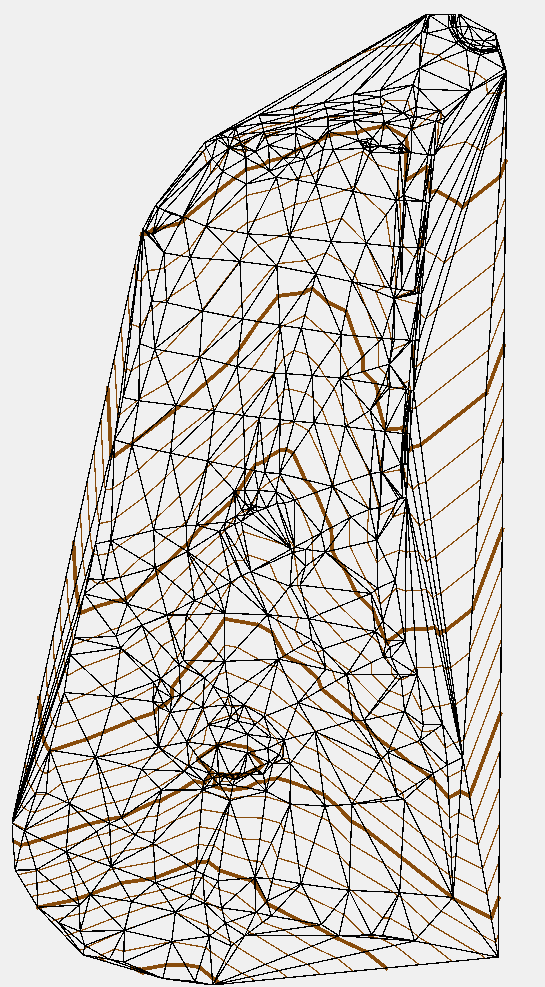
\includegraphics[scale=0.35]{images/chyba_nekonvex.png}
	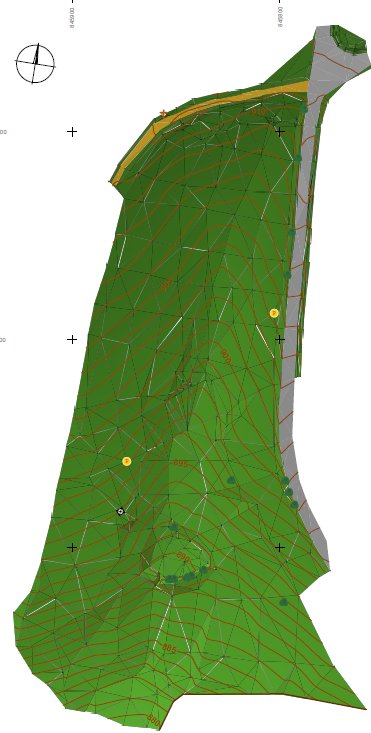
\includegraphics[scale=0.47]{images/chyba_nekonvex_spravne.png}
	\caption{Vrstevnice vykreslované mimo zájmové území - nekonvexní polygon}	
	\label{fig:nekonvex}
\end{figure} 
\FloatBarrier

Na následujícím obrázku je na levé straně nad údolím řeky Ohře vygenerována Delaunayho triangulace s vrstevnicemi, které chybně zasahují do vodního toku. Abychom tomu zabránily, je třeba kolem vodního toku zavést ostrovní hranu. Na pravě straně obrázku je pro porovnání uveden snímek ze ZMČR, kde jsou vrstevnice na vodním toku ošetřeny.

\clearpage

\begin{figure}[htbh]
	\centering
	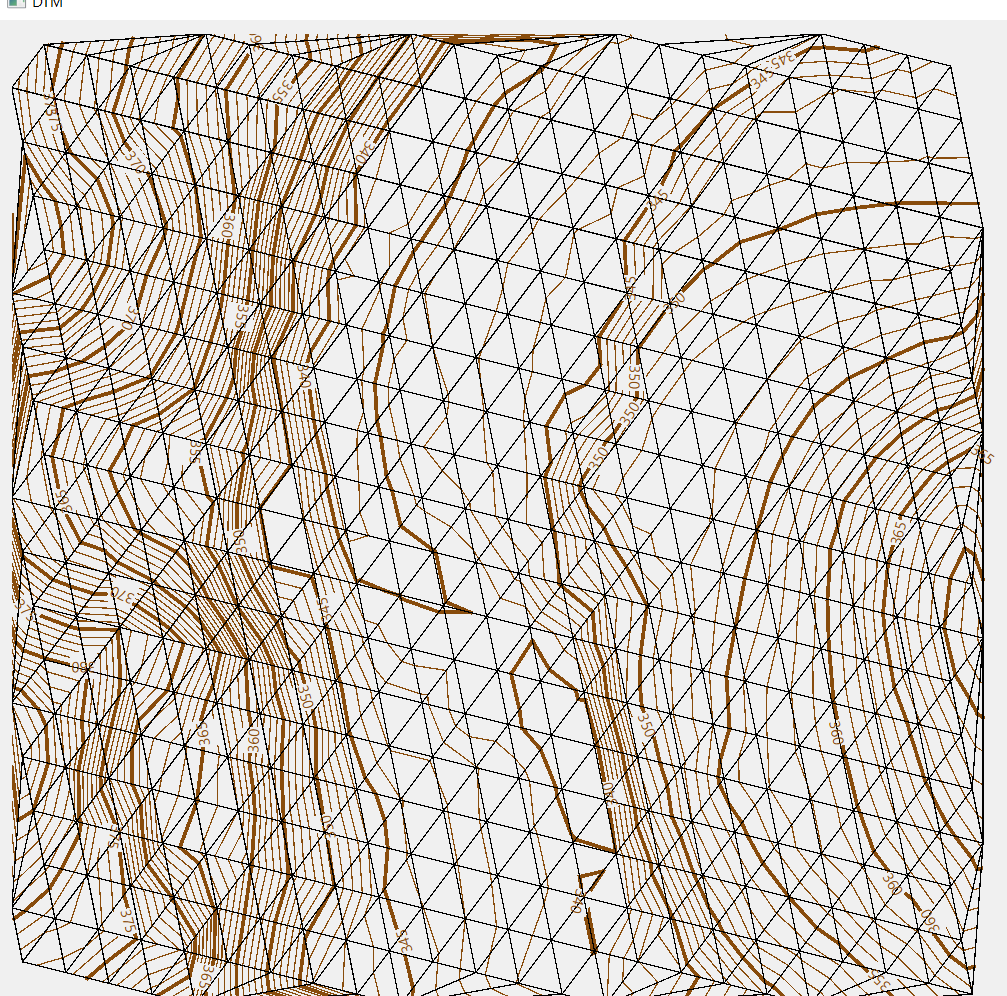
\includegraphics[scale=0.23]{images/chyba_reka.png}
	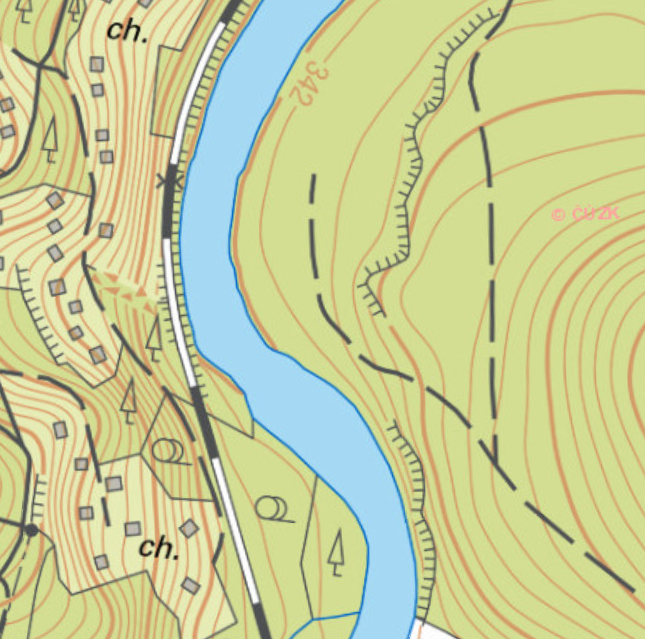
\includegraphics[scale=0.35]{images/chyba_reka_zm.png}
	\caption{Vrstevnice vykreslované přes řeku s chybějící ostrovní hranou}	
	\label{fig:reka}
\end{figure} 

Aplikace nabízí prostor pro mnoha zlepšení, avšak ve své aktuální verzi představuje funkční nástroj pro jednoduché výškové analýzy. 

\end{document}
